%%
%% This is file `sample-sigconf.tex',
%% generated with the docstrip utility.
%%
%% The original source files were:
%%
%% samples.dtx  (with options: `sigconf')
%% 
%% IMPORTANT NOTICE:
%% 
%% For the copyright see the source file.
%% 
%% Any modified versions of this file must be renamed
%% with new filenames distinct from sample-sigconf.tex.
%% 
%% For distribution of the original source see the terms
%% for copying and modification in the file samples.dtx.
%% 
%% This generated file may be distributed as long as the
%% original source files, as listed above, are part of the
%% same distribution. (The sources need not necessarily be
%% in the same archive or directory.)
%%
%% The first command in your LaTeX source must be the \documentclass command.
\documentclass[sigconf]{acmart}
\usepackage{listings}
\usepackage[justification=centering]{caption}

\lstset{language=C++,keywordstyle={\bfseries \color{blue}}}

%%
%% \BibTeX command to typeset BibTeX logo in the docs
\AtBeginDocument{%
  \providecommand\BibTeX{{%
    \normalfont B\kern-0.5em{\scshape i\kern-0.25em b}\kern-0.8em\TeX}}}

%% Rights management information.  This information is sent to you
%% when you complete the rights form.  These commands have SAMPLE
%% values in them; it is your responsibility as an author to replace
%% the commands and values with those provided to you when you
%% complete the rights form.
% \setcopyright{acmcopyright}
\copyrightyear{2019}
\acmYear{2019}
\acmDOI{PLEASE-DONT-CLICK-ME}

%% These commands are for a PROCEEDINGS abstract or paper.
\acmConference[CS259 Spring '19]{CS259: Final Project Report}{June 13, 2019}{Los Angeles, CA}

%%
%% Submission ID.
%% Use this when submitting an article to a sponsored event. You'll
%% receive a unique submission ID from the organizers
%% of the event, and this ID should be used as the parameter to this command.
%%\acmSubmissionID{123-A56-BU3}

%%
%% The majority of ACM publications use numbered citations and
%% references.  The command \citestyle{authoryear} switches to the
%% "author year" style.
%%
%% If you are preparing content for an event
%% sponsored by ACM SIGGRAPH, you must use the "author year" style of
%% citations and references.
%% Uncommenting
%% the next command will enable that style.
%%\citestyle{acmauthoryear}

%%
%% end of the preamble, start of the body of the document source.
\begin{document}
%%
%% The "title" command has an optional parameter,
%% allowing the author to define a "short title" to be used in page headers.
\title{Parallel Kernel Execution on GPUs}

%%
%% The "author" command and its associated commands are used to define
%% the authors and their affiliations.
%% Of note is the shared affiliation of the first two authors, and the
%% "authornote" and "authornotemark" commands
%% used to denote shared contribution to the research.
\author{Sahil Gandhi}
\authornote{Both authors contributed equally to this research.}
\email{sahilmgandhi@ucla.edu}
\author{Matthew Wong}
\email{mattwong949@ucla.edu}
\authornotemark[1]
\affiliation{%
  \institution{University of California, Los Angeles}
  \streetaddress{420 Westwood Plaza}
  \city{Los Angeles}
  \state{California}
}


%%
%% By default, the full list of authors will be used in the page
%% headers. Often, this list is too long, and will overlap
%% other information printed in the page headers. This command allows
%% the author to define a more concise list
%% of authors' names for this purpose.
\renewcommand{\shortauthors}{Gandhi and Wong, et al.}

%%
%% The abstract is a short summary of the work to be presented in the
%% article.
\begin{abstract}

While Moore’s law may be slowing down, GPU’s continue to get \textit{considerably} better with each generation. In 2010, Nvidia began to support executing multiple kernels at once (concurrently), initially allowing only 4-16 kernels to be executed concurrently but increasing it to 128 today. Kernels and machine learning problems that used to take up all the resources of a GPU several years ago now only take a fraction of compute power. In this report, we specifically focus on comparing the concurrent execution of kernels to their sequential counterparts to investigate whether the overhead of launching kernels in parallel defeats any performance gains from the concurrency we are exploiting. We also compare these kernels to their batched versions, the industry norm for maximizing performance. 

The results that we obtained suggest that concurrent kernel execution can increase performance anywhere from 1.25x to 15x, with smaller problems seeing larger performance gains. For smaller problems, batched kernels beat the performance of concurrent kernels greatly, but for large problems, the performances are approximately the same with concurrent kernels actually being about 5\% to 10\% faster. Our findings suggest that if there is a level of parallelism that can be added, such as in the classifier where not all dimensions of threads are used, concurrent kernels can provide performance on par or even better than batched kernels. Combined with the the paper of \textit{Jiao et al.} where concurrent kernels provided almost 34.5\% better energy efficiency, perhaps these may be the future of running many kernels \cite{jiao_lu_huynh_mitra_2015}. Furthermore, concurrent kernel execution may be used over batching is if different types of problems were mixed together, as batching requires all the batches to be of the same size/type, but heterogeneous kernels can be concurrently executed.
\end{abstract}

%%
%% The code below is generated by the tool at http://dl.acm.org/ccs.cfm.
%% Please copy and paste the code instead of the example below.
%%
\begin{CCSXML}
<ccs2012>
 <concept>
  <concept_id>10010520.10010553.10010562</concept_id>
  <concept_desc>Computer systems organization~Embedded systems</concept_desc>
  <concept_significance>500</concept_significance>
 </concept>
 <concept>
  <concept_id>10010520.10010575.10010755</concept_id>
  <concept_desc>Computer systems organization~Redundancy</concept_desc>
  <concept_significance>300</concept_significance>
 </concept>
 <concept>
  <concept_id>10010520.10010553.10010554</concept_id>
  <concept_desc>Computer systems organization~Robotics</concept_desc>
  <concept_significance>100</concept_significance>
 </concept>
 <concept>
  <concept_id>10003033.10003083.10003095</concept_id>
  <concept_desc>Networks~Network reliability</concept_desc>
  <concept_significance>100</concept_significance>
 </concept>
</ccs2012>
\end{CCSXML}

% \ccsdesc[500]{Computer systems organization~Embedded systems}
% \ccsdesc[300]{Computer systems organization~Redundancy}
% \ccsdesc{Computer systems organization~Robotics}
% \ccsdesc[100]{Networks~Network reliability}

%%
%% Keywords. The author(s) should pick words that accurately describe
%% the work being presented. Separate the keywords with commas.
% \keywords{datasets, neural networks, gaze detection, text tagging}

%% A "teaser" image appears between the author and affiliation
%% information and the body of the document, and typically spans the
%% page.
% \begin{teaserfigure}
%   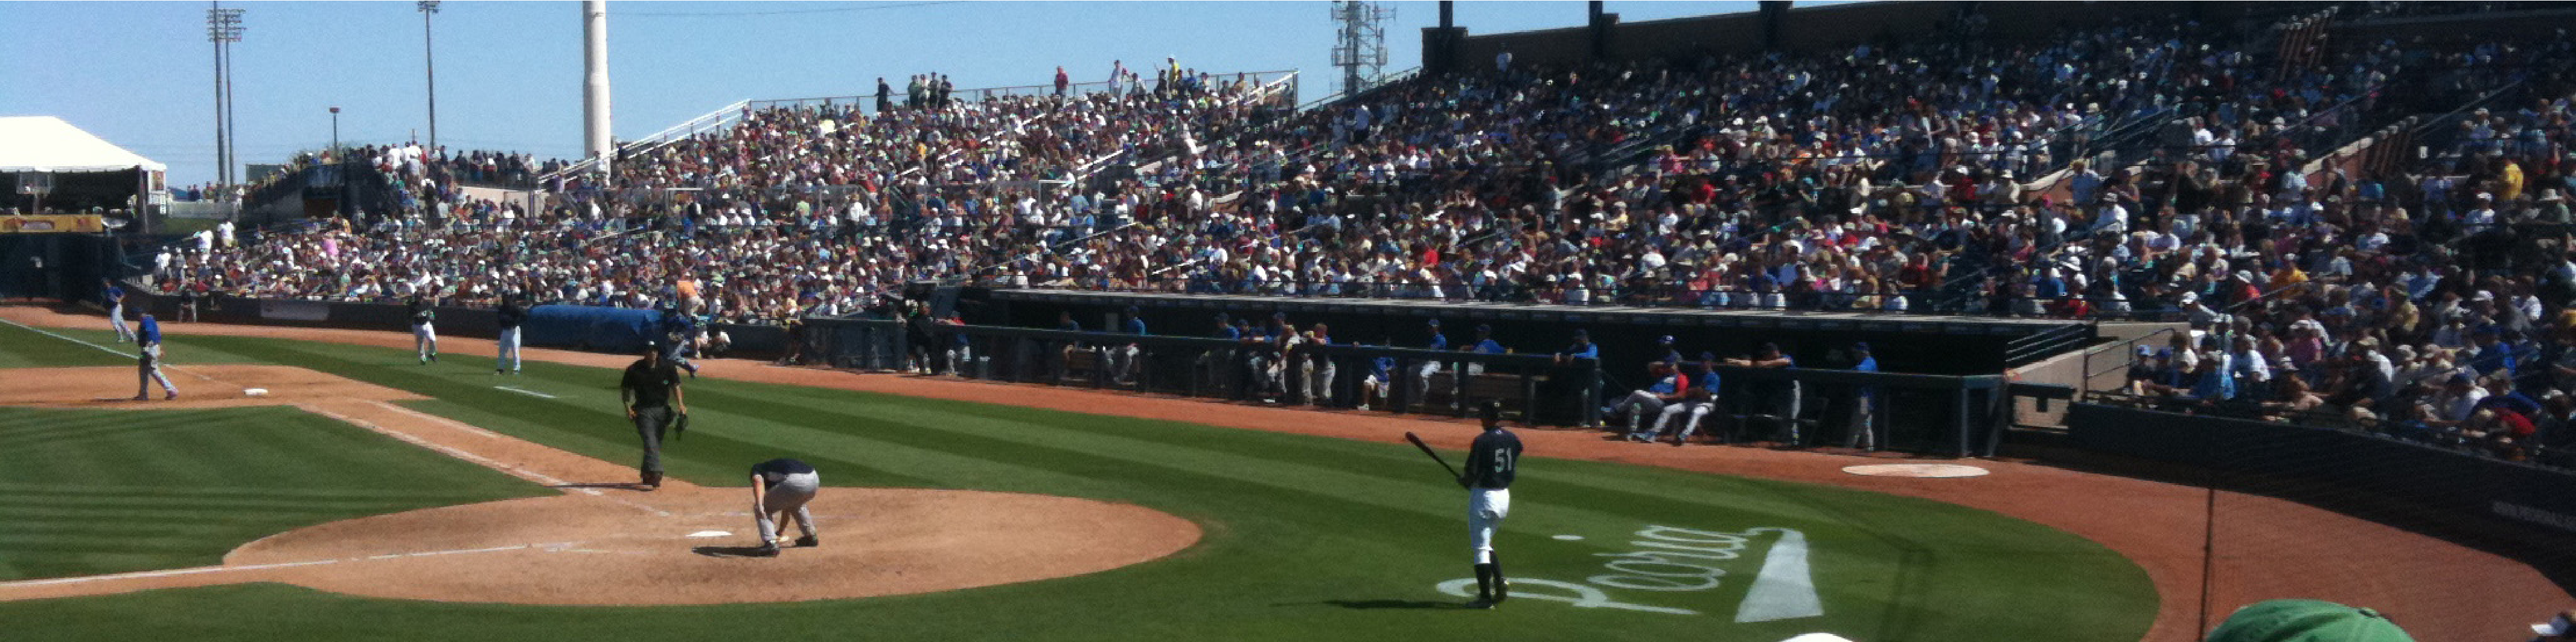
\includegraphics[width=\textwidth]{sampleteaser}
%   \caption{Seattle Mariners at Spring Training, 2010.}
%   \Description{Enjoying the baseball game from the third-base
%   seats. Ichiro Suzuki preparing to bat.}
%   \label{fig:teaser}
% \end{teaserfigure}

%%
%% This command processes the author and affiliation and title
%% information and builds the first part of the formatted document.
\maketitle

\section{Introduction}
As GPUs become more powerful and start packing more cores and SMs, problems that previously used up an entire GPU now only use a fraction of them. Consider the Nvidia Quadro Plex 2200 from four generations ago with 648 cores, the Nvidia M4 GPU from only two generations ago which packed 1024 cores, and the Tesla V100 that has 5120 cores \cite{nvidia_all_gpus}. Every generation nearly doubles the amount of cores that are available, and Nvidia continues to offer other enhancements such as Tensor cores to increase the performance of the graphics cards. 

One such enhancement is the ability to concurrently execute kernels, which was introduced in 2010 with the Fermi architecture. Prior to this, kernels had to be queued up sequentially, and only after a kernel had finished all of its computation, would the next one get an opportunity to start. At the start, only 16 kernels could be concurrently executed - though Nvidia profiled that in reality it appeared only 4 were truly concurrent due to hardware issues - today we can expect up to 128 kernels to be concurrently executed. The implications of this technology are that we no longer have to wait for kernels to finish before executing other work on the GPU, which is particularly important if the GPU is not being fully utilized by one kernel or is being shared by different developers/teams. Furthermore, unlike batching where all of the kernels are of the same type or may be sharing data, concurrent kernels can be heterogeneous and work on independent workloads. 

This report intends to dive deep into the practicality and functionality of using concurrent kernels for some well known kernels such as convolution layers and classification layers. The lack of support and other related works suggests that concurrent kernels may not be as powerful or useful as they seem. However, we want to confirm or reject this notion with our own data, and hope that others can build off of it to parametrize kernels that can be run concurrently and deliver performances that are on par or better than the current industry norm of batching jobs together.  


\section{Related Work}
As aforementioned, Nvidia first introduced the concept of concurrent kernel execution about nine years ago with their Fermi architecture. Their “Streams and Concurrent Webinar” powerpoint from 2010 explains the gist of using them and shows some cases as to when this may be helpful (notably when there are small problems that can be run in parallel to utilize more of the GPU) \cite{nvidia_concurrent}. Since then, there have been some other developments in the research community that have explored topics such as the energy efficiency for concurrent kernels, sharing data between concurrent kernels, the proper ordering of kernels to maximize utilization and more. 

\textit{Wang et al.} in 2011 first explored the notion of concurrent kernels and directly compared it to the sequential execution of kernels of varying block/thread sizes \cite{wang_huang_el_ghazawi_2011}. On the Nvidia Fermi architecture which supported 16 concurrent kernels (4 true concurrent kernels), they saw that if they just queued kernels with single blocks, the concurrent kernel implementation delivered anywhere between 10 to 16x better performance, but if they kept a fixed number of kernels and varied the block sizes, the performance between concurrent and sequential kernel execution was approximately the same with concurrent kernels winning only by anywhere between 0 - 20\%.

\textit{Wende et al.} in 2012 looked into the proper ordering of kernels to maximize performance \cite{wende_cordes_steinke_2012}. They found that by using a producer-consumer model for splitting up their work, they could get anywhere from 5x to 10x improvement to sequential kernels with their concurrent implementation. Furthermore in their experimentation on Fermi Nvidia GPUs, they noticed that as the number of blocks per kernel increased (their GPU had 8 SMs available), their overall performance quickly decreased from a full 16x speedup when each kernel used 1 block to 1.5x speedup when each kernel used 6 or more blocks. This matches the behavior that was observed in \textit{Wang et al.}.

\textit{Pai et al.} in 2013 worked on the concurrent kernels problem with a newer GPU, the Nvidia Kepler card that had 16 SMs, and also explored using “elastic-kernels”, kernels that were more aware of shared memory and synchronization between kernels \cite{pai_thazhuthaveetil_govindarajan_2013}. They observed that for a specific set of benchmarks, the Parboil 2 suite, an elastic concurrent kernel implementation could outperform a naive concurrent kernel implementation by 3.73x. However, they do not compare it to a regular sequential kernel implementation, so there is no basic benchmark to compare their results to. 

\textit{Jiao et al.} in 2015 was directed towards improving the energy efficiency of GPUs as in recent years, the TDP required from GPUs has been increasing steadily, with the failure of Dennard Scaling being imminent \cite{jiao_lu_huynh_mitra_2015}. Their trials on a variety of different kernel pairs in from an assortment of benchmarks showed that by using a DVFS (Dynamic Voltage Frequency Scaling) with the concurrent kernel method gave rise to 34.5\% better energy efficiency compared to the best sequential kernel execution method. This suggests that the concurrent kernel execution may indeed have other benefits than merely providing more throughput. 

\textit{Greg et al.} in 2016 attempted to create a scheduler for two kernels executing concurrently in OpenCL \cite{gregg_dorn_hazelwood_skadron_2016}. While their work is only for two kernels, they have shown that a proper ordering of kernels results in 39\% better performance than a naive ordering, and intend to create a more dynamic scheduler in the future that can support more kernels. 

There are a couple of patterns that we can observe from the above papers. First, concurrent kernels have not been researched in recent years when GPUs have gotten considerably larger than most non-batched kernel sizes. It is quite possible that today the results could be starkly different than they were in the past. Second, no one has actually compared the performance to batching, which is surprising as it is quite rare for companies to use a GPU for a single convolution or classification problem (perhaps an ASIC instead to minimize latency). We hope to explore this comparison in this report, and present our observations.

\section{Methods}

After going through the related work and Nvidia documentation/Stackoverflow posts we broke down our design pipeline and workflow as follows. For reference, we are using the Tesla V100 GPU which supports 80 SM that have 64 cores (for a total of 5120 cores), and has Compute 7.0 capability that allows it to run up to 128 concurrent kernels \cite{nvidia_spec}. 

\subsection{Exploring Streams and Concurrent Kernels}
The first thing we did was to test an initial implementation of concurrent kernels on a simple convolution layer. Since the kernel execution api is asynchronous, we thought that if we just queued up multiple kernels in a row without calling \lstinline{CudaDeviceSynchronize();}, the different kernels would run as soon as the asynchronous call finished. After writing several different kernels and running our profiling script, we saw that there was no difference in the execution time or the performances of the sequential and concurrent kernel implementations. We were shocked as the papers that we read suggested that we should start to see some performance gains (at the very least 1.1x-1.5x), especially if we are now running on a much more powerful GPU that can support many more concurrent kernels. We went back to the drawing board and the sdk examples and came upon the cudaStream api.

Cuda assigns each data source and kernel into a data stream which its scheduler can then queue up to the GPU, transfer the data, and start the computation. There is a certain amount of overhead that occurs here, about 10 us to schedule a kernel and 4 us to execute it \cite{michaelmichael}. By default there is one stream that all kernels are placed within, and only one kernel can run in a stream at a time, so even without that \lstinline{CudaDeviceSynchronize();}, multiple kernels in a row would run sequentially. However multiple streams can be executed concurrently, and if each stream is assigned one or more kernels, then you can have concurrent kernel execution. A code example is given below. 

\begin{figure}[h]
  \centering
  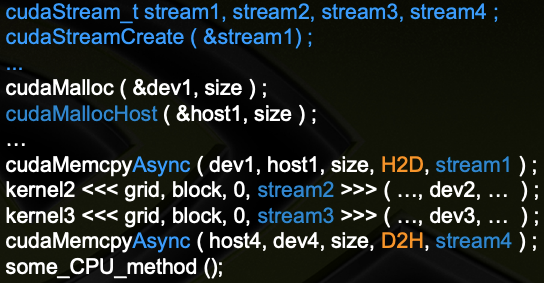
\includegraphics[width=\linewidth]{img/image1}
  \caption{Cuda streams API example. Taken from the Nvidia Concurrent Kernel PowerPoint. \cite{nvidia_concurrent}}
\end{figure}

\begin{figure}[h]
  \centering
  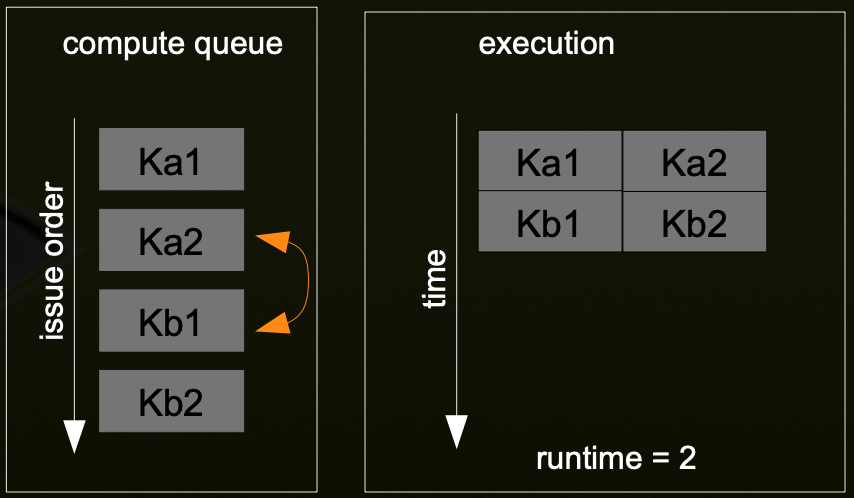
\includegraphics[width=\linewidth]{img/image6}
  \caption{Cuda concurrent kernel execution schedule. Taken from the Nvidia Concurrent Kernel PowerPoint. \cite{nvidia_concurrent}}
\end{figure}

Furthermore, the order that the streams are queued up is the order in which the kernels are executed, so below we can see that if we have 2 streams with 2 kernels each (ka1/kb1 and ka2/kb2) and if we put Ka1 and Ka2 back-to-back, then both can be simultaneously executed. Kb1/kb2 will be executed after the first kernels finish. 

\subsection{Creating a Set of Kernels	}
The next step was to create a set of kernels to run concurrently. Since we had a rather large GPU, we figured that we could test a range of kernels of different sizes to see how the concurrent kernels would affect performance. We created two kernels, a convolution layer kernel and a classifier layer kernel. The convolution kernel had 64, 128, and 256 blocks with 1024, 2048 and 4096 threads in total respectively. The classifier kernel had 2,4,8,16,32,64, and 128 blocks with 64, 128, 256, 512, 1024, 2048 and 4096 threads in total respectively. These kernels are all rather large, but we noticed that at any point in time, we would have no more than 10-20\% of the threads actually running at once due to memory access latencies requiring warps to be swapped. Thus we were confident that unlike some of the experiments by \cite{wende_cordes_steinke_2012} where concurrent kernels with more threads resulted in negligible performance gains, we should see some noticeable improvement. 

Furthermore, it is important to note that the blocking, tiling, and shared memory parameters we chose for both of the kernels are not the most optimal. We consciously chose to do this as we cannot expect every engineer to have the most fine tuned kernels in the world, and we were unsure if Cudnn supported a concurrent kernel implementation (to serve as a benchmark). Our convolution kernel was parallelized across three dimensions of threads, and used shared memory. Meanwhile our classifier kernel was parallelized only across one dimension of threads and used tiling heavily. These will be key parameters to keep in mind when we talk about batched kernels in a later section. 

\subsection{Profiling Latency and Throughput}

To calculate the latency and throughput of the kernels, we timed the execution for the computation part of the kernel (we did not time the memory transfers) and calculated the total number of computations ($Nn*Ni*2*Nb$ and $nxpad*nypad*Nb*Nn*Ni*Ky*Kx*2$ for classifier and convolution respectively, where Nb = number of kernels) and divided it by time, respectively. We created a bash script to run through all of the different sizes of kernels and outputted the latency and throughput results to a csv file so that we could graph it. All of the different profiling scripts take about 8-10 hours in total to run, with the convolution ones taking about 1-2 hours each and classifier ones taking 3-4 hours each. We ran the convolution kernels for 1,2,4,6, ... 20 concurrent kernels and the classifier kernels for 1,2,4,6, ... 20, 30, 40, 50, 60 concurrent kernels. 

\subsection{Creating Batched Kernels}
Finally, we observed that none of the related works compared the concurrent kernel execution performances to the batched kernel variant that is the industry norm today. We thus modified our kernels to support batching. For the classifier kernel, we could just add another dimension of threads and surround the old kernel code with a \lstinline{for} loop to go through the different batches. For the convolution though, we had to move one of the dimensions of threads from being used on the output layer to being used on the \lstinline{for} surrounding the old kernel code. We re-profiled the sequential and concurrent performances for this new convolution kernel to make a fare comparison. Furthermore, we used the same number of batches as concurrent kernels above (1,2,4,6, ... 20 for convolution and 1,2,4,6, ... 20, 30, 40, 50, 60 for classifier).

\section{Methodology}
To evaluate our work, we took many different kernel sizes and batch-sizes/concurrent-counts, and profiled the latency and throughput for them using our shell scripts. We tried to get a wide range of kernel sizes and kernel counts to see how different workloads would affect the performance. Primarily we were looking to see the point where we would no longer see any improvement with concurrent or batched kernels since the GPU would be fully utilized, and were also trying to observe the diminishing speedup reported by \textit{Wende et al.} when kernels got very large \cite{wende_cordes_steinke_2012}. 

Due to the two different convolutions that we had to create, we did not have a fair comparison between the concurrent execution for conv1 and the concurrent execution for conv2 since an entire dimension of parallelism was missing from conv2 (since we had to use those threads instead for the batched version of the kernel). Thus the performances for conv2 are significantly lower than those for conv1, and the batched version for conv2 is naturally better than the concurrent or sequential conv2 implementations.

Furthermore, as aforementioned, our classifier and convolution kernels are not the most optimized kernels. We chose to keep them relatively un-optimized since we wanted to observe how different block/thread counts would affect the final performance when running sequentially vs concurrently vs when batched. A fully optimized kernel that used far more of the GPU with a batch size of 1 may not see the same performance gains that we observed for the concurrent/batched runs since there are not many resources left on the GPU to divide amongst more kernels. 

Finally, to make our evaluation a bit more general, we decided to also run our kernels on an Nvidia M60 GPU on the AWS g3s.xlarge instance. This GPU has 16 SMs that we can use, for a total of 1024 cores, so it is about 1/5 the size of the Tesla V100 that we had available from the professor. The results that we got from testing on this GPU are quite different from the V100 GPU results (to say the least), and we will briefly touch on them in the evaluation section below. 

\section{Evaluation}
To not clutter the report, we have added all the graphs to the appendix of this report.

\subsection{Sequential vs Concurrent Convolution 1}
The sequential execution of the first convolution kernel we implemented increased linearly in execution time as the number of kernels increased. Also, the GFLOPS stayed constant for all input and output sizes that we tested. In other words, the GFLOPS was independent of the number of kernels being executed, which is logical for a sequential implementation where the GFLOPS should neither be increasing nor decreasing. 

The concurrent execution of the same convolution kernel performed much faster than sequential execution. We observed speedup of execution time in the range of 5x - 15x for the different test cases that we were profiling. This resulted in a much higher maximum throughput of 750 GFLOPS for concurrent execution versus the 300 GFLOPS for sequential execution. We conclude that concurrent execution of the kernels had larger utilization of the GPU’s cores and other resources, since concurrent kernels could be switched in while others were waiting to hide latency of memory accesses. However, we also notice that the throughput drops when the number of kernels increases past the peak throughput. We reason that the GPU resources become saturated after this point, and executing more kernels concurrently cannot raise utilization any further. Instead, the overhead of launching and managing more kernels increases total latency of context switches, decreasing throughput.


\subsection{Sequential vs Concurrent vs Batched Convolution 2}

We implemented a second convolution kernel that was capable of batching, and ran the same sequential and concurrent tests that we had profiled for the first convolution kernel. We also ran the same tests in a batched version, in which only one kernel would be executed to run all work that normally would have been distributed across multiple kernels.

In comparing the sequential and concurrent executions of this second convolution, we notice similar patterns to that of the first convolution. Sequential execution increased linearly with respect to the number of kernels, and GFLOPS stayed mostly consistent, unaffected by the number of kernels. The sequential execution had odd spikes of performance when the number of kernels was low, which we could not explain and was probably due to other factors we could not control within Cuda or the GPU. Aside from this, the concurrent execution times were faster than sequential, achieving speedup in the range of 1.4x - 2x. The throughput of this second convolution was similar in trend to that of the first convolution, since it also peaked at a maximum before dropping as number of kernels increased. Again, we reason that the causes for this drop are saturation of GPU resources and overhead of concurrent kernels.

The batched execution of this convolution had much higher performance than the concurrent version did, achieving as much as 8x speedup for most batch sizes. The maximum throughput peaked at about 600 GFLOPS, linearly increasing as the number of batches increased. This is a notable difference compared to concurrent and sequential executions, which seem to plateau or fall with increasing number of kernels. There is no overhead of launching and managing multiple kernels, and all of the GPU’s resources are allocated to this single kernel. As batch size increases, the kernel has more computation to distribute among blocks, allowing for efficient GPU utilization. It is noted that this throughput is lower than the first concurrent-convolution’s maximum throughput of 750 GFLOPs. However, to give this second convolution the ability to perform on batches, we removed a level of parallelism that the kernel could have distributed among thread blocks, so it is not a fair comparison.

\subsection{Sequential vs Concurrent vs Batched Classifier}

We also implemented a classifier layer on which we could run profiling tests. We wanted to see if similar results would be seen with a different type of kernel. For sequential execution, we notice that execution time increases linearly as the number of kernels increases, similar to the convolution results. Likewise, the throughput seems to plateau with the increasing number of kernels. This is reasonable since sequential execution should not increase throughput.

Comparing sequential and concurrent executions of the classifier layer, we notice that some of the execution times of concurrent kernels were slower than the sequential counterparts. For test cases with smaller input and output sizes, concurrent kernels were able to produce speedup in the range of 1.5x - 2.0x. This allowed the maximum throughput on concurrent kernels to achieve 150 GFLOPS compared to the sequential maximum of 100 GFLOPS. However, for test cases with larger sizes, concurrent execution was slower than sequential execution. We reason that the overhead of concurrent execution was much greater than executing sequentially. Since the classifier kernel was not optimized, data reuse was also not optimized. We suspect that the concurrent kernels were competing for memory resources when the problem size became too large, increasing latency of memory reads beyond what could be hidden by concurrency. Sequential kernels did not encounter this overhead, allowing them to finish faster. 

The batched execution of the classifier resulted in approximately the same performance as the concurrent kernel implementation for the four larger kernel sizes. In fact, for these four larger kernel sizes, the concurrent classifier actually performed about 5\% to 10\% better than the batched versions. However for the smaller three problem sizes, the batched classifier almost 2x better as the number of batches went up. This suggests that the few microseconds of overhead for the smaller problems that is introduced in the concurrent implementation affects the overall performance considerably (since the execution time here is also in the order of microseconds). Batching does not suffer from this overhead since only one kernel is ever queued and launched. However what is more important about this conclusion is that for classification layers, we see that concurrent kernels can provide equivalent if not better performance and are thus worth a deeper investigation on some of the state of the art kernels (such as CUDNN).


\subsection{AWS M60 Results}
We ran all of our profiling scripts with the same number of blocks and batch counts for the different kernels on an AWS g3s.xlarge instance. While the GPU is considerably weaker than the Tesla V100 GPU, the results are not as impressive or as conclusive (but still not completely inconclusive either) as with the ones discussed above. 
  
For convolution 1, the concurrent kernel implementation is about 1.2x - 1.4x faster than the sequential implementation but it quickly saturates within the first concurrent 4-6 kernels that were executed. This lines up quite similarly to the results of \textit{Wende et al.} where they only saw 1.2x improvement with concurrent kernels if the kernels had more than 1 block worth of work to do. Our kernels for convolution had between 64 and 256 blocks to compute, so the results match up \cite{wende_cordes_steinke_2012}. 
  
For convolution 2, we see that the concurrent kernel implementation initially performs about 2x better than the sequential version until 6 kernel mark after which the performance quickly dives to be the same as the sequential version. This intuitively does not make sense, as even if the GPU is fully saturated or over saturated it should still deliver performance that is larger than the purely sequential version. The batched implementation does not suffer from this though as the performance for batched conv2 continues to increase as the number of batches increased till the 18 batch mark before falling slightly as the GPU got over saturated. Despite this drop, it still provided more than 6x throughput than the sequential and concurrent kernel versions at 20 batches.
  
For the classifier, we observed that the for the larger problems, the concurrent, sequential and batched kernels all resulted in the same performance. However the smaller problems sizes saw noticeable improvement with the concurrent and batched offering approximately the same performance (2x to 5x better than the sequential kernel implementation).

\section{Conclusion}
In conclusion, we can see that concurrent kernel execution is a pretty powerful tool that for certain problems can provide comparable or better performance to batching. We saw anywhere between 1.5x to 15x throughput improvement from switching from sequential to concurrent kernel execution. With the classifier, we saw approximately the same performance between concurrent and batched kernels, suggesting that for problems with limited amounts of memory re-use and large overall memory requirements, the two methods can provide comparable performance. We saw however with the second convolution kernel that the batched variant provided anywhere between 2x to 8x better performance over the concurrent variant. This was likely due to the kernel being severely under-optimized after we took out one of the dimensions of threads from the original convolution problem. Although it is not a fair comparison to make, we can see that the batched conv2 performance is actually lower than the concurrent kernel performance for conv1 by about 1.2 - 1.4x. Overall though, it seems like concurrent kernel execution can be a worthy contender to the batched kernel execution that is the industry norm today. 

For future ideas in expanding this work, we considered several different paths. One idea was looking into heterogeneous sets of kernels. As we mentioned earlier, batching requires the same type of kernel to be executed. Thus, with sets of individually unique kernels, batching to increase performance is no longer an option. Concurrent execution is the next option, for which we could investigate the performance gains. Another idea was investigating CUDNN to see if we could modify it for concurrent kernel execution. If the modifications were possible, we could profile the fully-optimized kernels and measure the performance changes.
  
Currently, we only considered performance gains in computation from executing kernels concurrently. However, there are multiple parts to consider when running on the GPU, such as copying memory to the device (H2D) and copying the results back from the device (D2H). These memory copies can be executed asynchronously by working in conjunction with cudaStream objects. Considering performance gains from concurrently performing memory copies and computation, would inflate our results, but is still worth investigating.

We also were unable to investigate how Tensor cores would affect the performance. Tensor cores are limited in numbers, kind of like how SMs were in the past, so we could quickly saturate our supply of them with even a couple kernels. However, a future investigation could confirm or reject this hypothesis.


\section{Statement of Work}
Both Matt and Sahil split the work roughly equally, with the two of us working on different parts of the report and presentation, creating the different kernels and shell scripts and analyzing the results.

All code can be found at the following link: \url{https://github.com/sahilmgandhi/cs-259-final-project}.


% \begin{itemize}
% \item the ``ACM Reference Format'' text on the first page.
% \item the ``rights management'' text on the first page.
% \item the conference information in the page header(s).
% \end{itemize}


% \section{Tables}

% The ``\verb|acmart|'' document class includes the ``\verb|booktabs|''
% package --- \url{https://ctan.org/pkg/booktabs} --- for preparing
% high-quality tables.

% Table captions are placed {\itshape above} the table.

% Because tables cannot be split across pages, the best placement for
% them is typically the top of the page nearest their initial cite.  To
% ensure this proper ``floating'' placement of tables, use the
% environment \textbf{table} to enclose the table's contents and the
% table caption.  The contents of the table itself must go in the
% \textbf{tabular} environment, to be aligned properly in rows and
% columns, with the desired horizontal and vertical rules.  Again,
% detailed instructions on \textbf{tabular} material are found in the
% \textit{\LaTeX\ User's Guide}.

% Immediately following this sentence is the point at which
% Table~\ref{tab:freq} is included in the input file; compare the
% placement of the table here with the table in the printed output of
% this document.

% \begin{table}
%   \caption{Frequency of Special Characters}
%   \label{tab:freq}
%   \begin{tabular}{ccl}
%     \toprule
%     Non-English or Math&Frequency&Comments\\
%     \midrule
%     \O & 1 in 1,000& For Swedish names\\
%     $\pi$ & 1 in 5& Common in math\\
%     \$ & 4 in 5 & Used in business\\
%     $\Psi^2_1$ & 1 in 40,000& Unexplained usage\\
%   \bottomrule
% \end{tabular}
% \end{table}

% To set a wider table, which takes up the whole width of the page's
% live area, use the environment \textbf{table*} to enclose the table's
% contents and the table caption.  As with a single-column table, this
% wide table will ``float'' to a location deemed more
% desirable. Immediately following this sentence is the point at which
% Table~\ref{tab:commands} is included in the input file; again, it is
% instructive to compare the placement of the table here with the table
% in the printed output of this document.

% \begin{table*}
%   \caption{Some Typical Commands}
%   \label{tab:commands}
%   \begin{tabular}{ccl}
%     \toprule
%     Command &A Number & Comments\\
%     \midrule
%     \texttt{{\char'134}author} & 100& Author \\
%     \texttt{{\char'134}table}& 300 & For tables\\
%     \texttt{{\char'134}table*}& 400& For wider tables\\
%     \bottomrule
%   \end{tabular}
% \end{table*}

%% The next two lines define the bibliography style to be used, and
%% the bibliography file.
\bibliographystyle{ACM-Reference-Format}
\bibliography{bibliography}

\newpage
%%
%% If your work has an appendix, this is the place to put it.
\appendix

\section{Appendices}

In order to not clutter the report above, we added all the images of the graphs below. The first section contains the 
images for the Tesla V100 GPU, and the second for the M60 GPU. 

\subsection{Tesla V100 GPU Graphs}

\begin{figure}[htb]
  \centering
  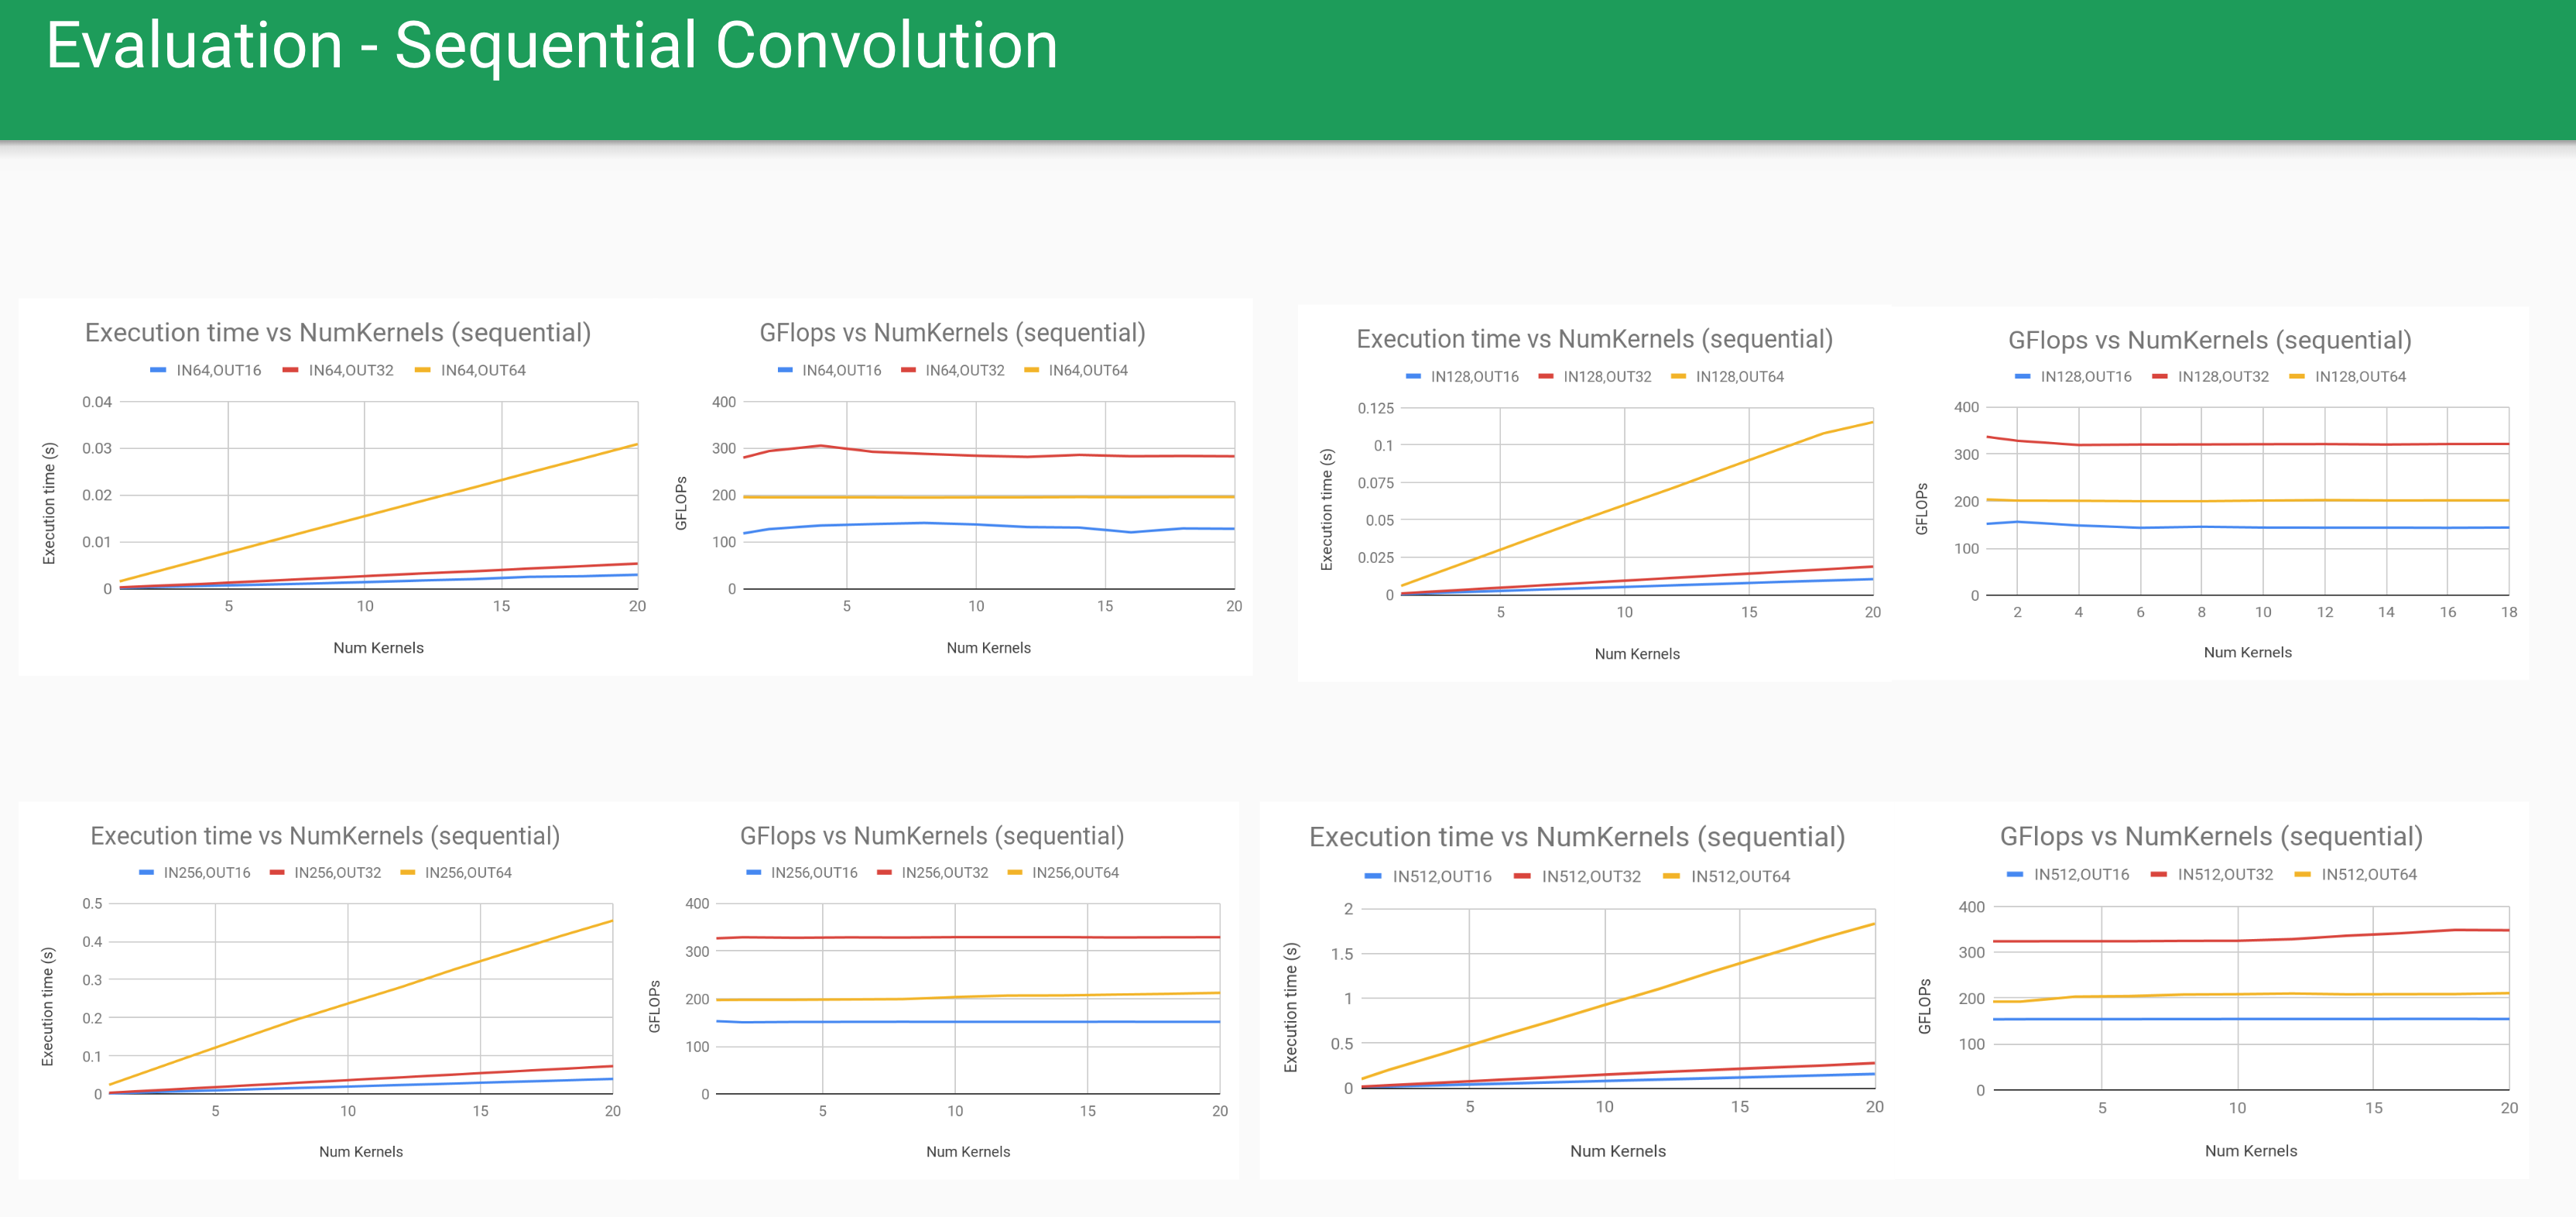
\includegraphics[width=\textwidth]{img/seq-conv}
  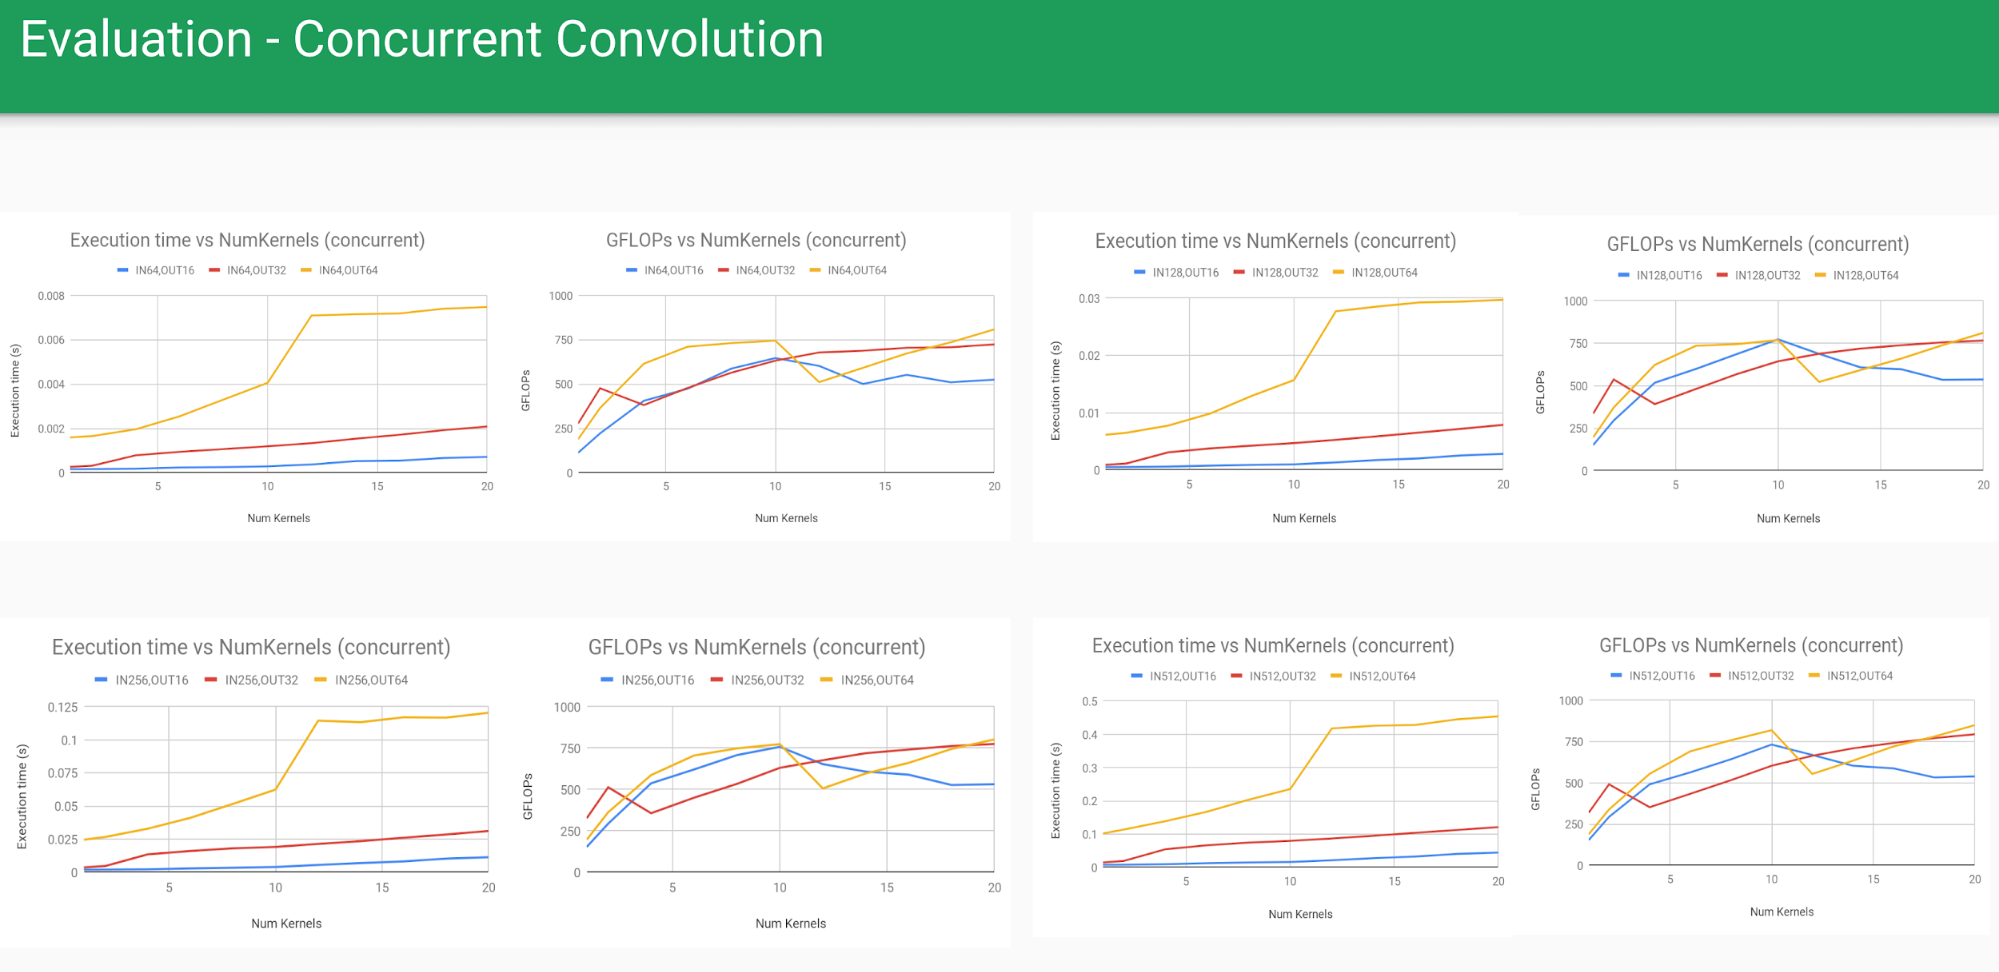
\includegraphics[width=\textwidth]{img/conc-conv}
  \caption{Sequential and concurrent convolution performance.}
\end{figure}

\newpage~\newpage
\begin{figure}[htb]
  \centering
  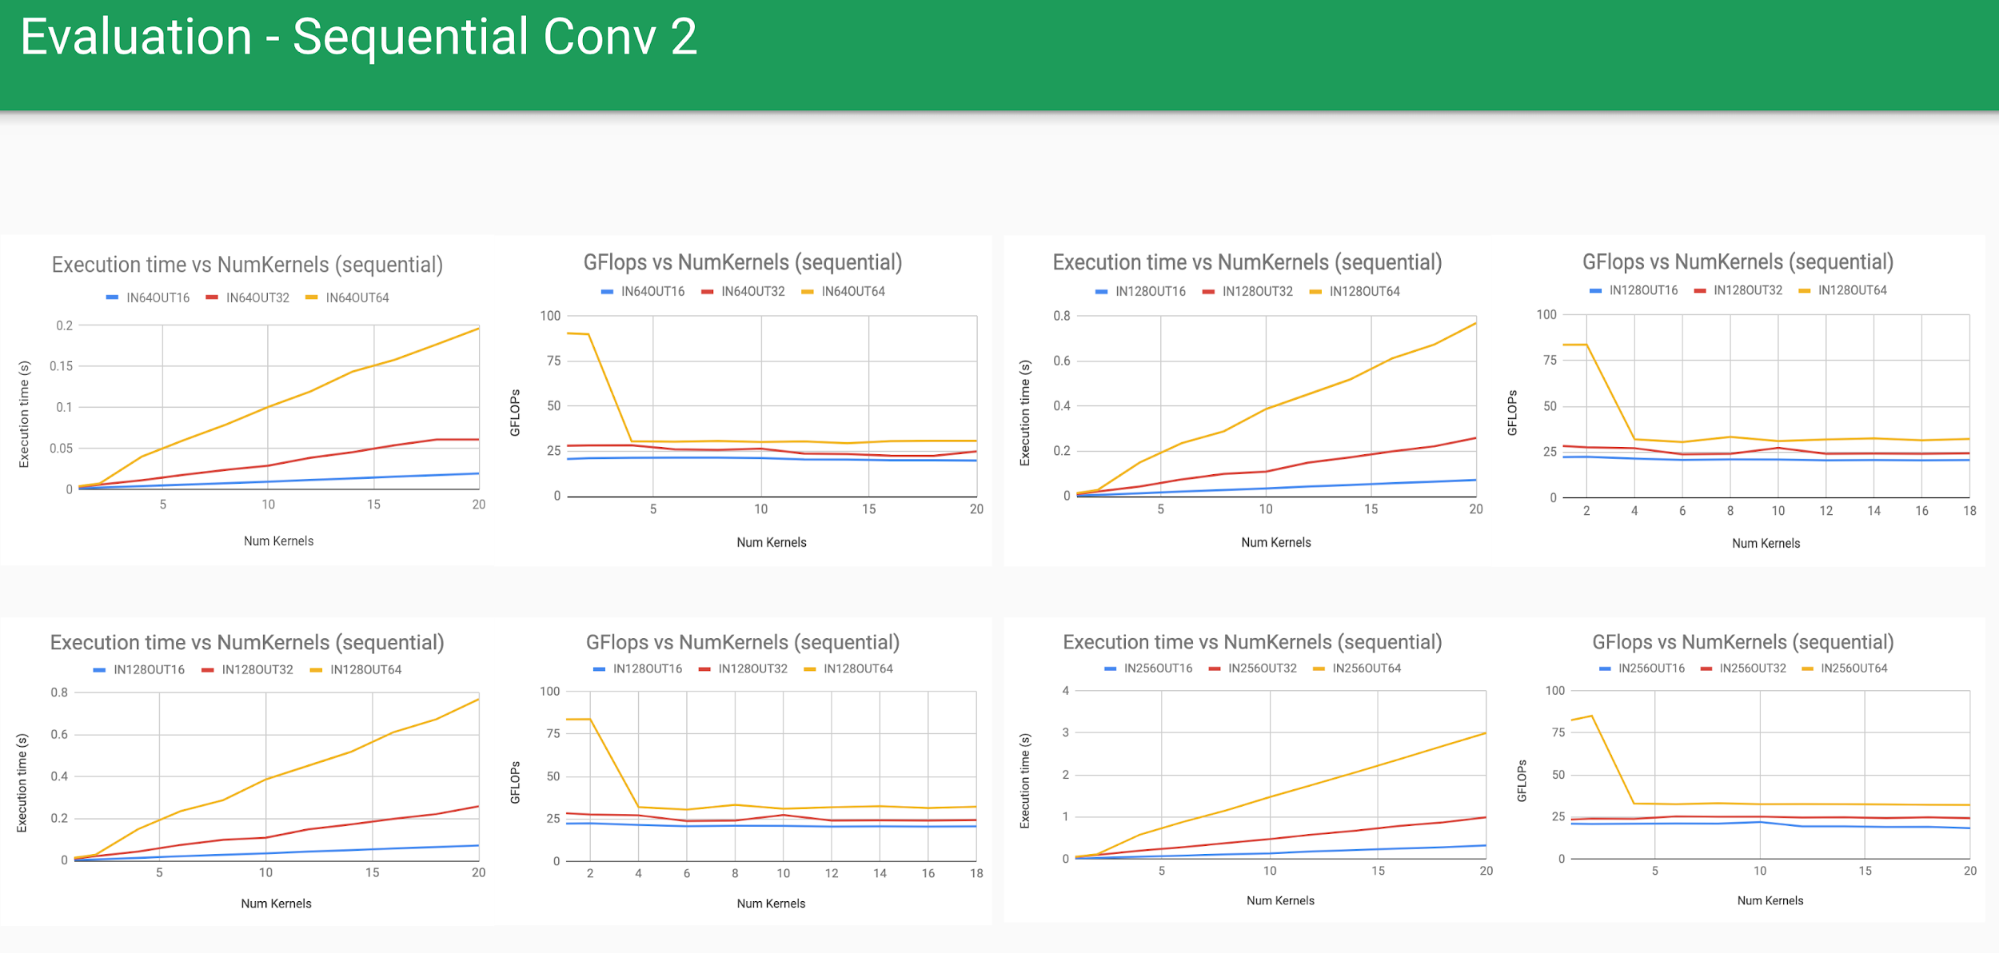
\includegraphics[width=\textwidth]{img/seq-conv2}
  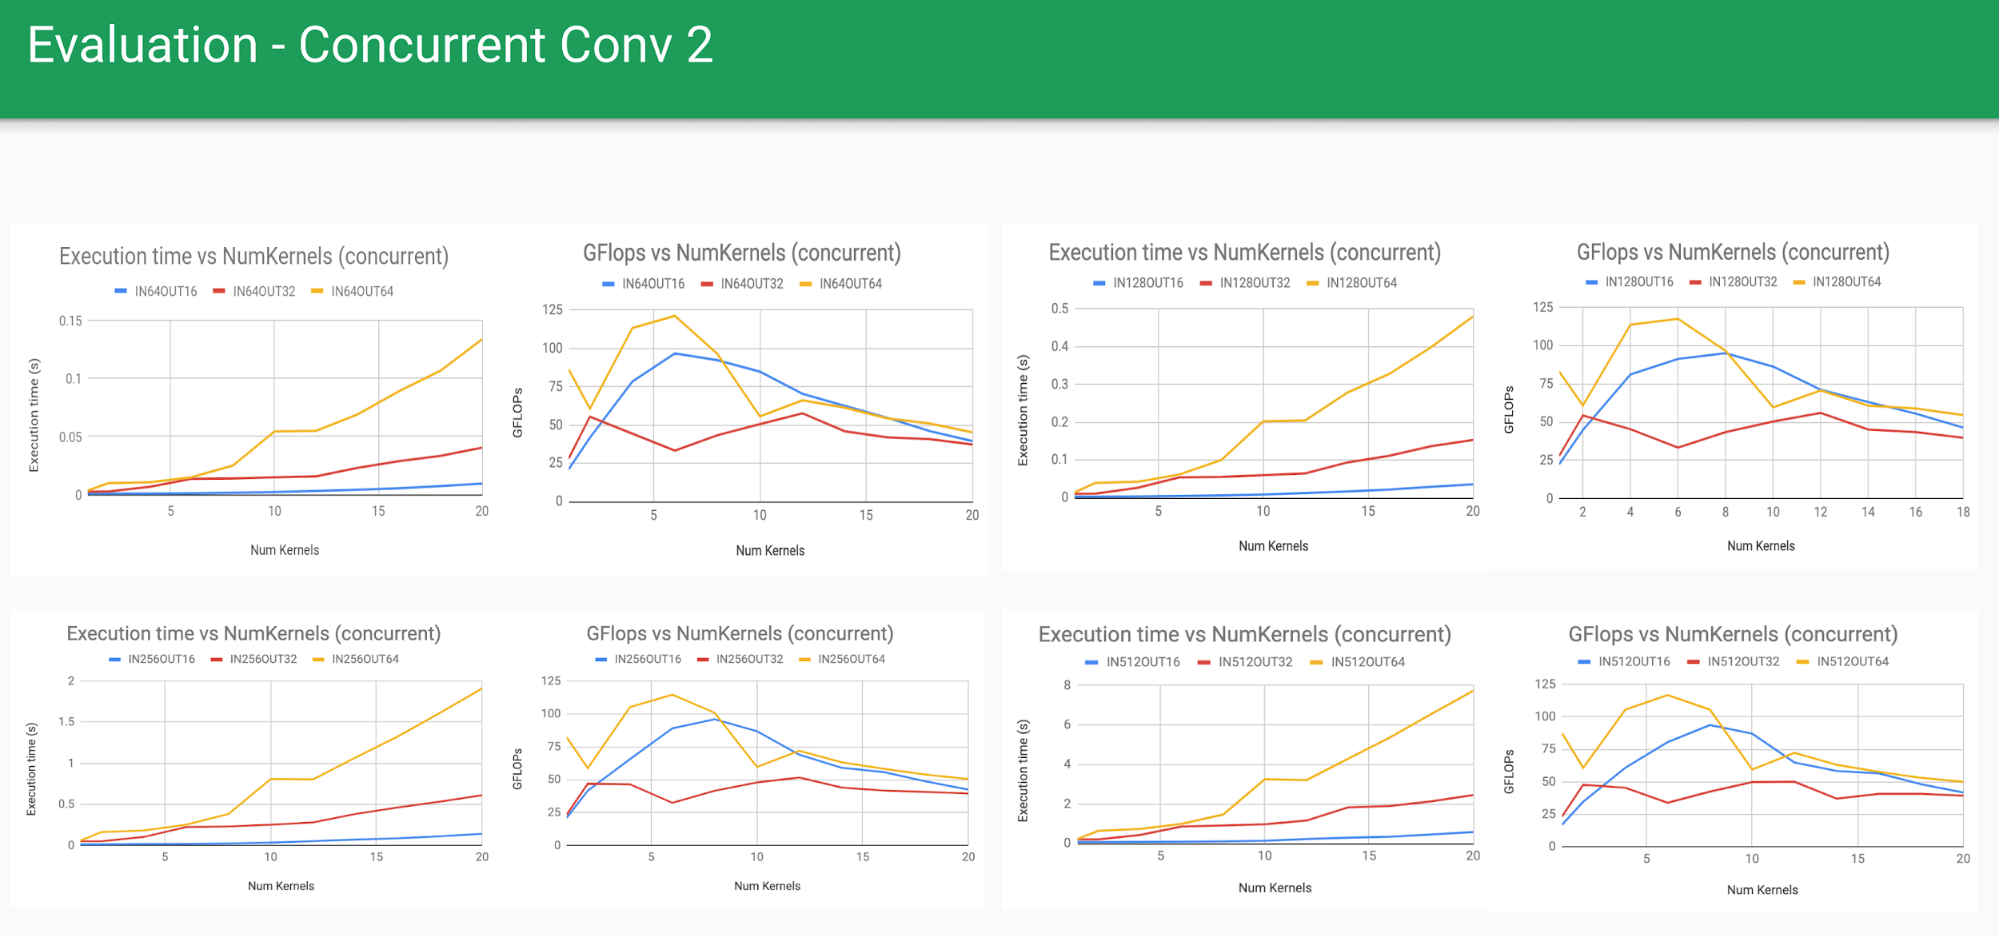
\includegraphics[width=\textwidth]{img/conc-conv2}
  \caption{Sequential and concurrent convolution 2 performance.}
\end{figure}

\newpage~\newpage
\begin{figure}[htb]
  \centering
  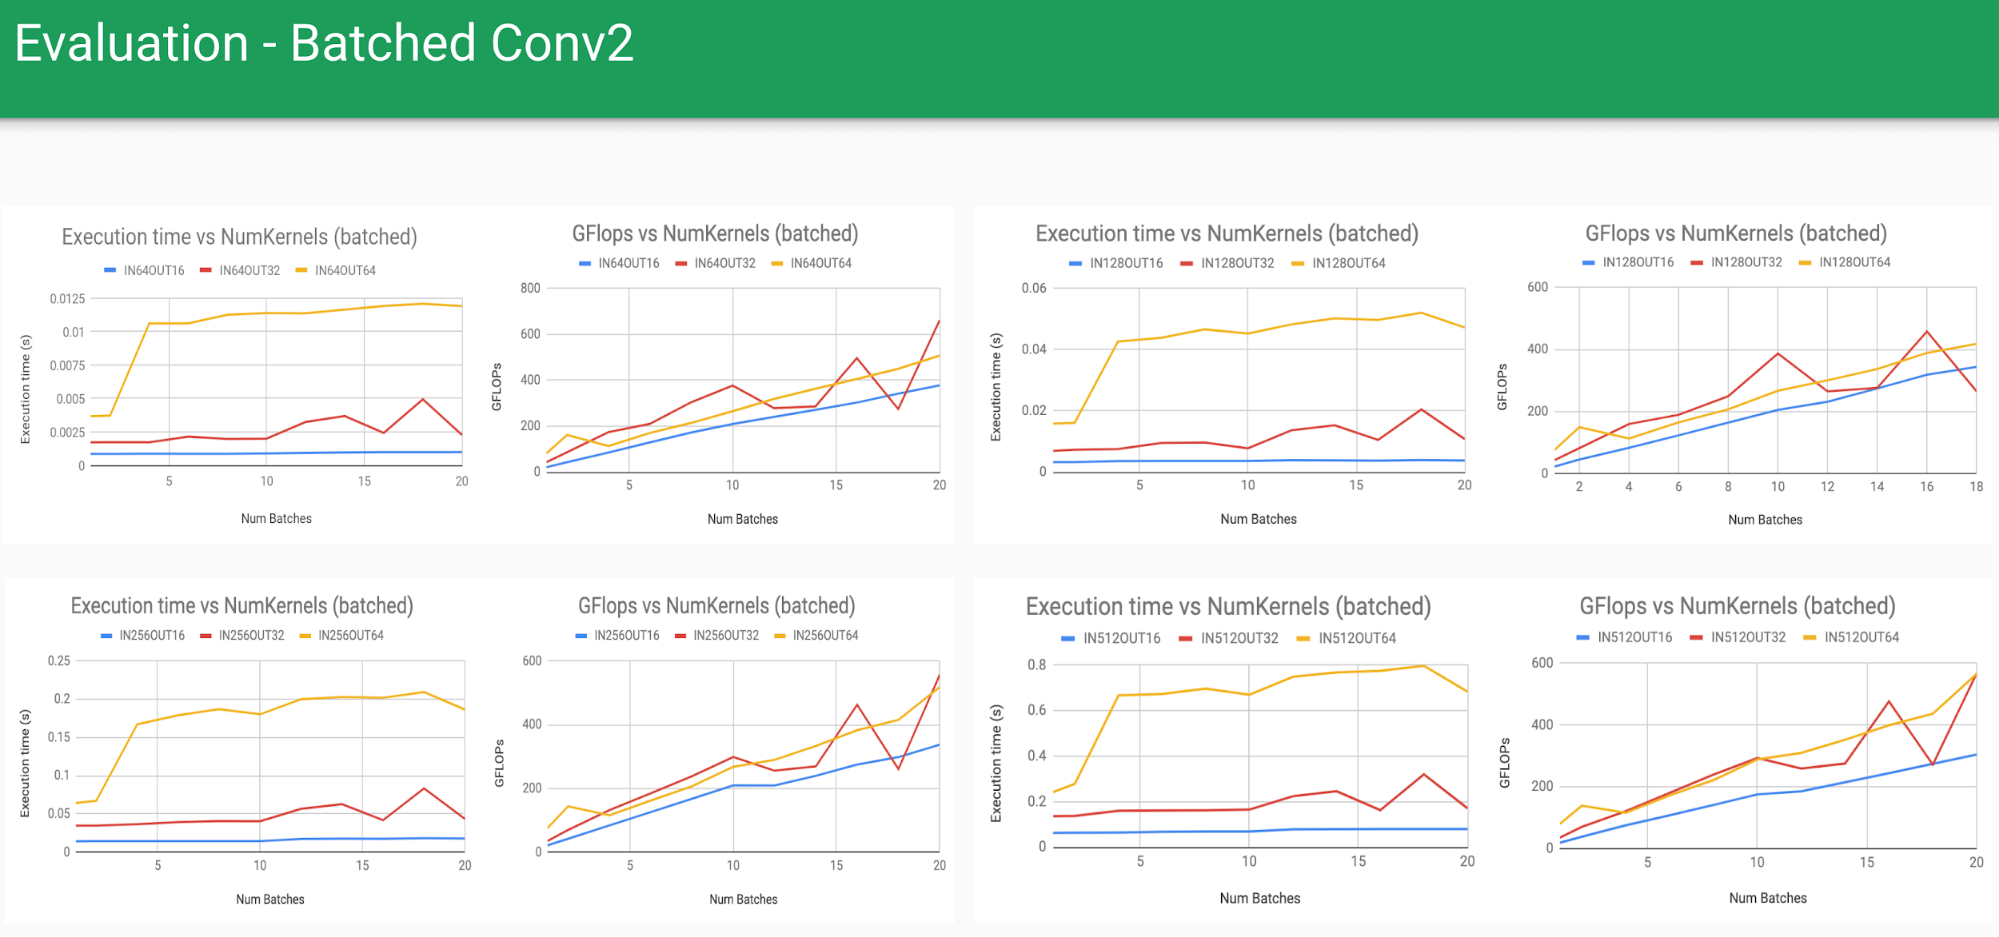
\includegraphics[width=\textwidth]{img/batch-conv2}
  \caption{Batched convolution 2 performance.}
\end{figure}

\newpage~\newpage
\begin{figure}[htb]
  \centering
  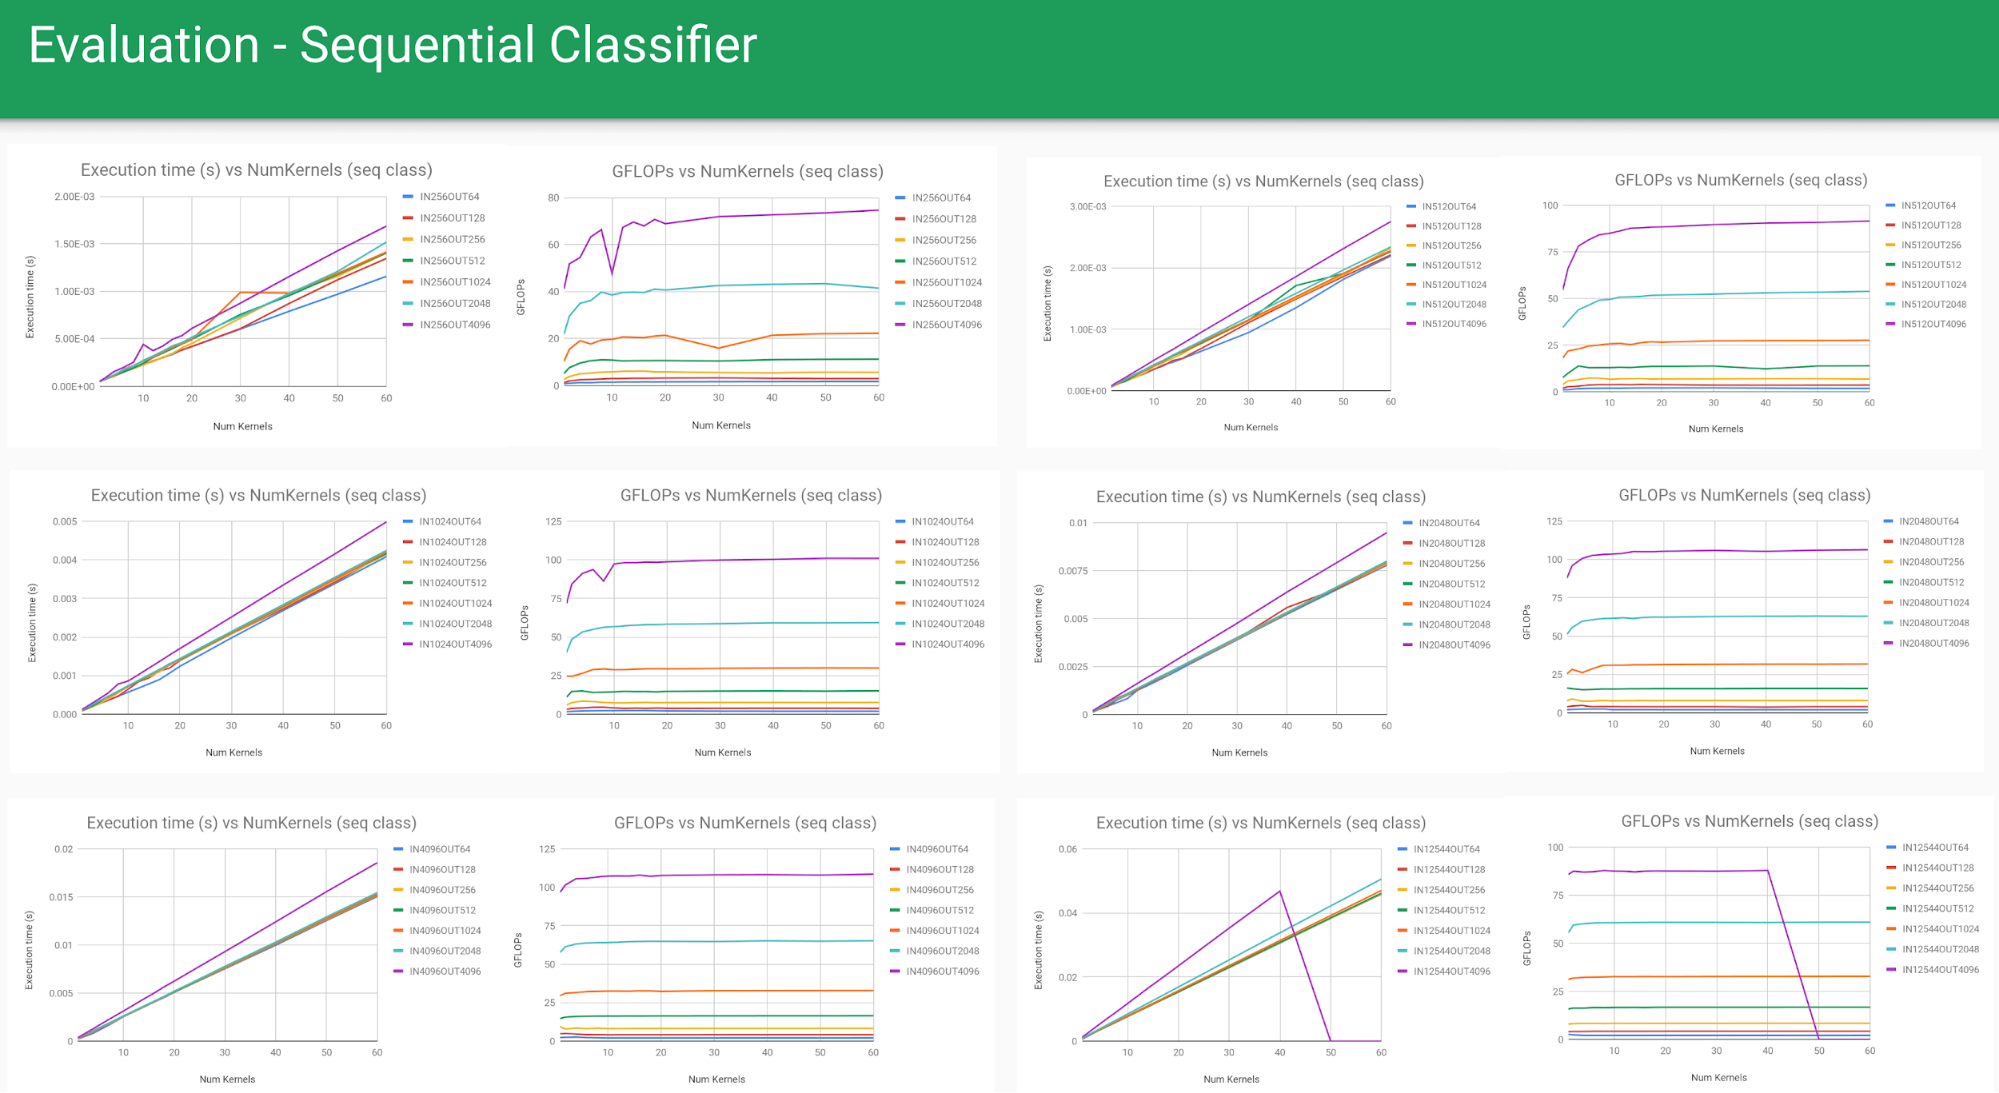
\includegraphics[width=\textwidth]{img/seq-class}
  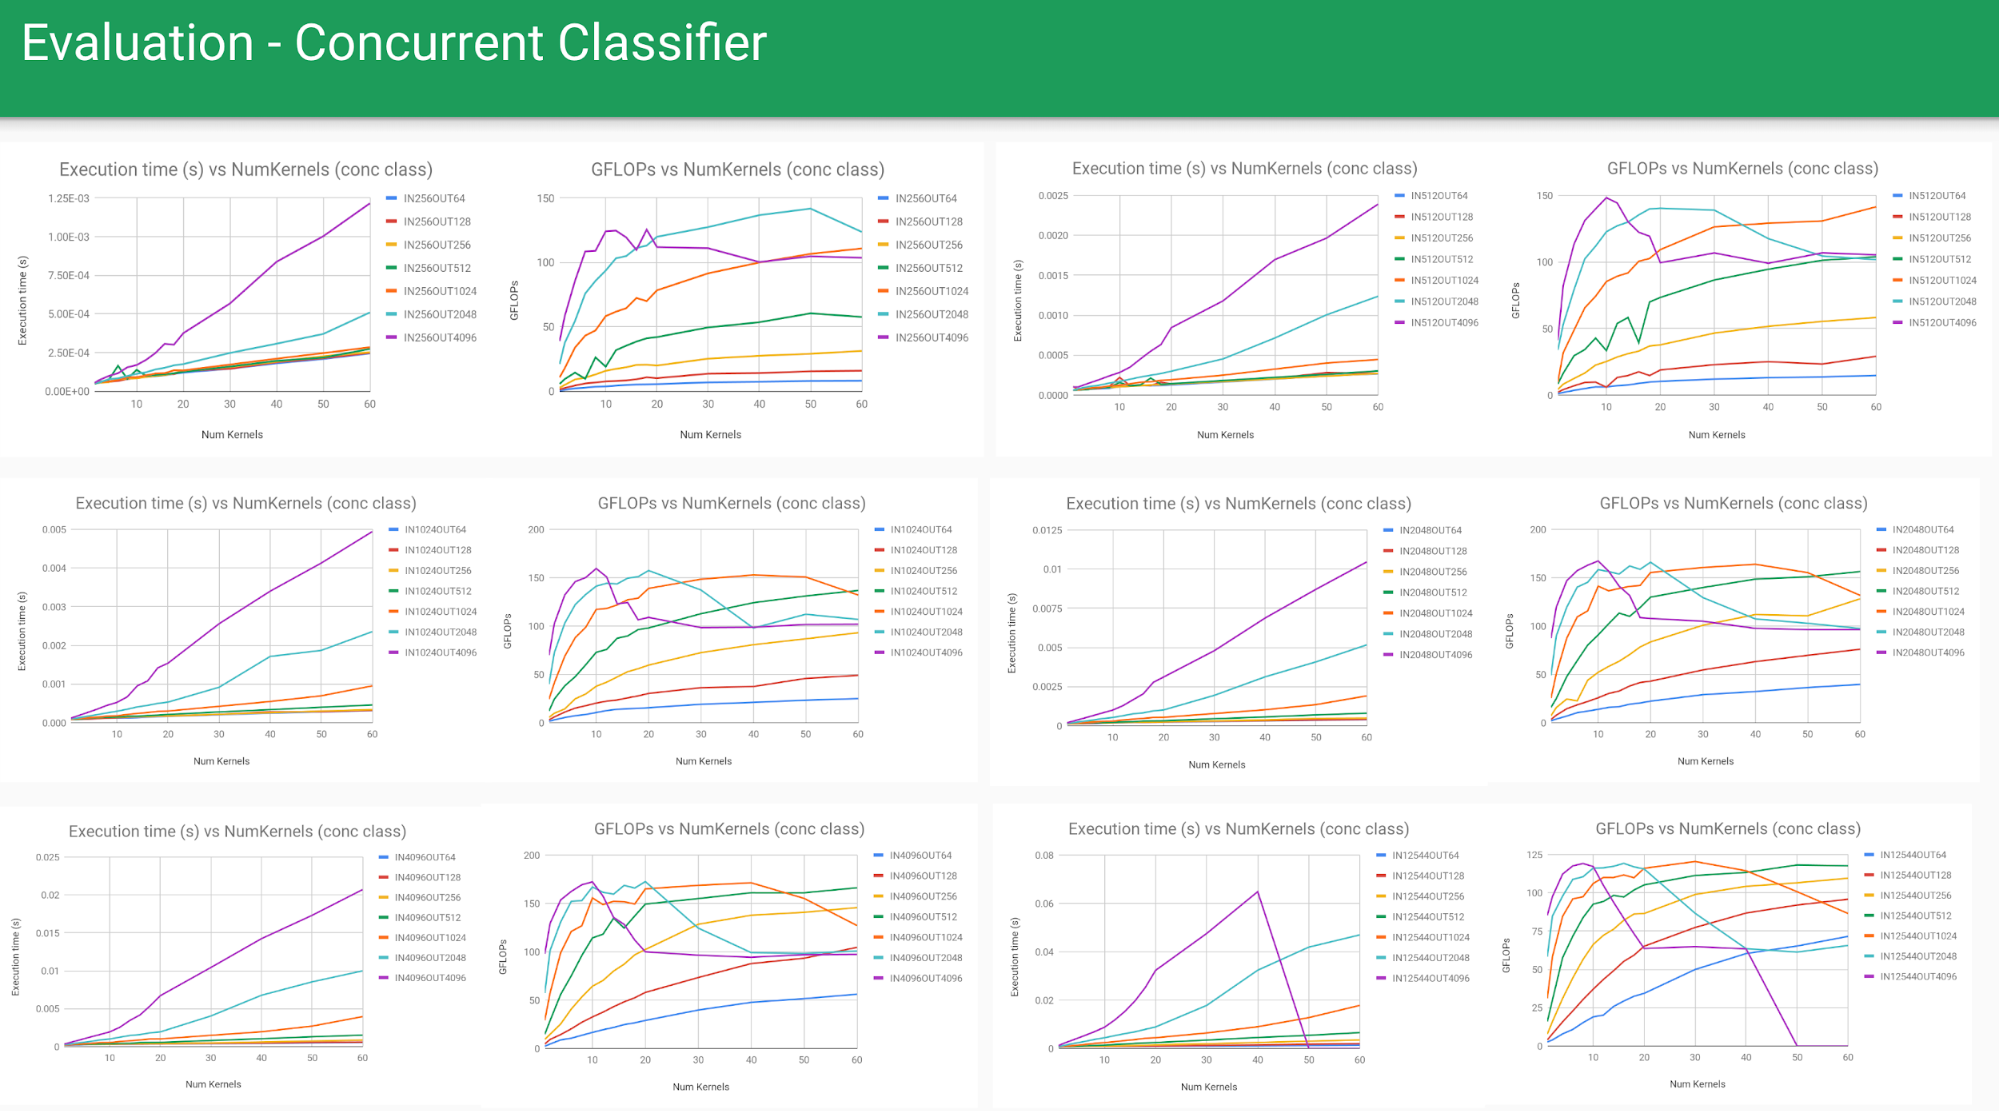
\includegraphics[width=\textwidth]{img/conc-class}
  \caption{Sequential and concurrent classifier performance.}
\end{figure}

\newpage~\newpage
\begin{figure}[htb]
  \centering
  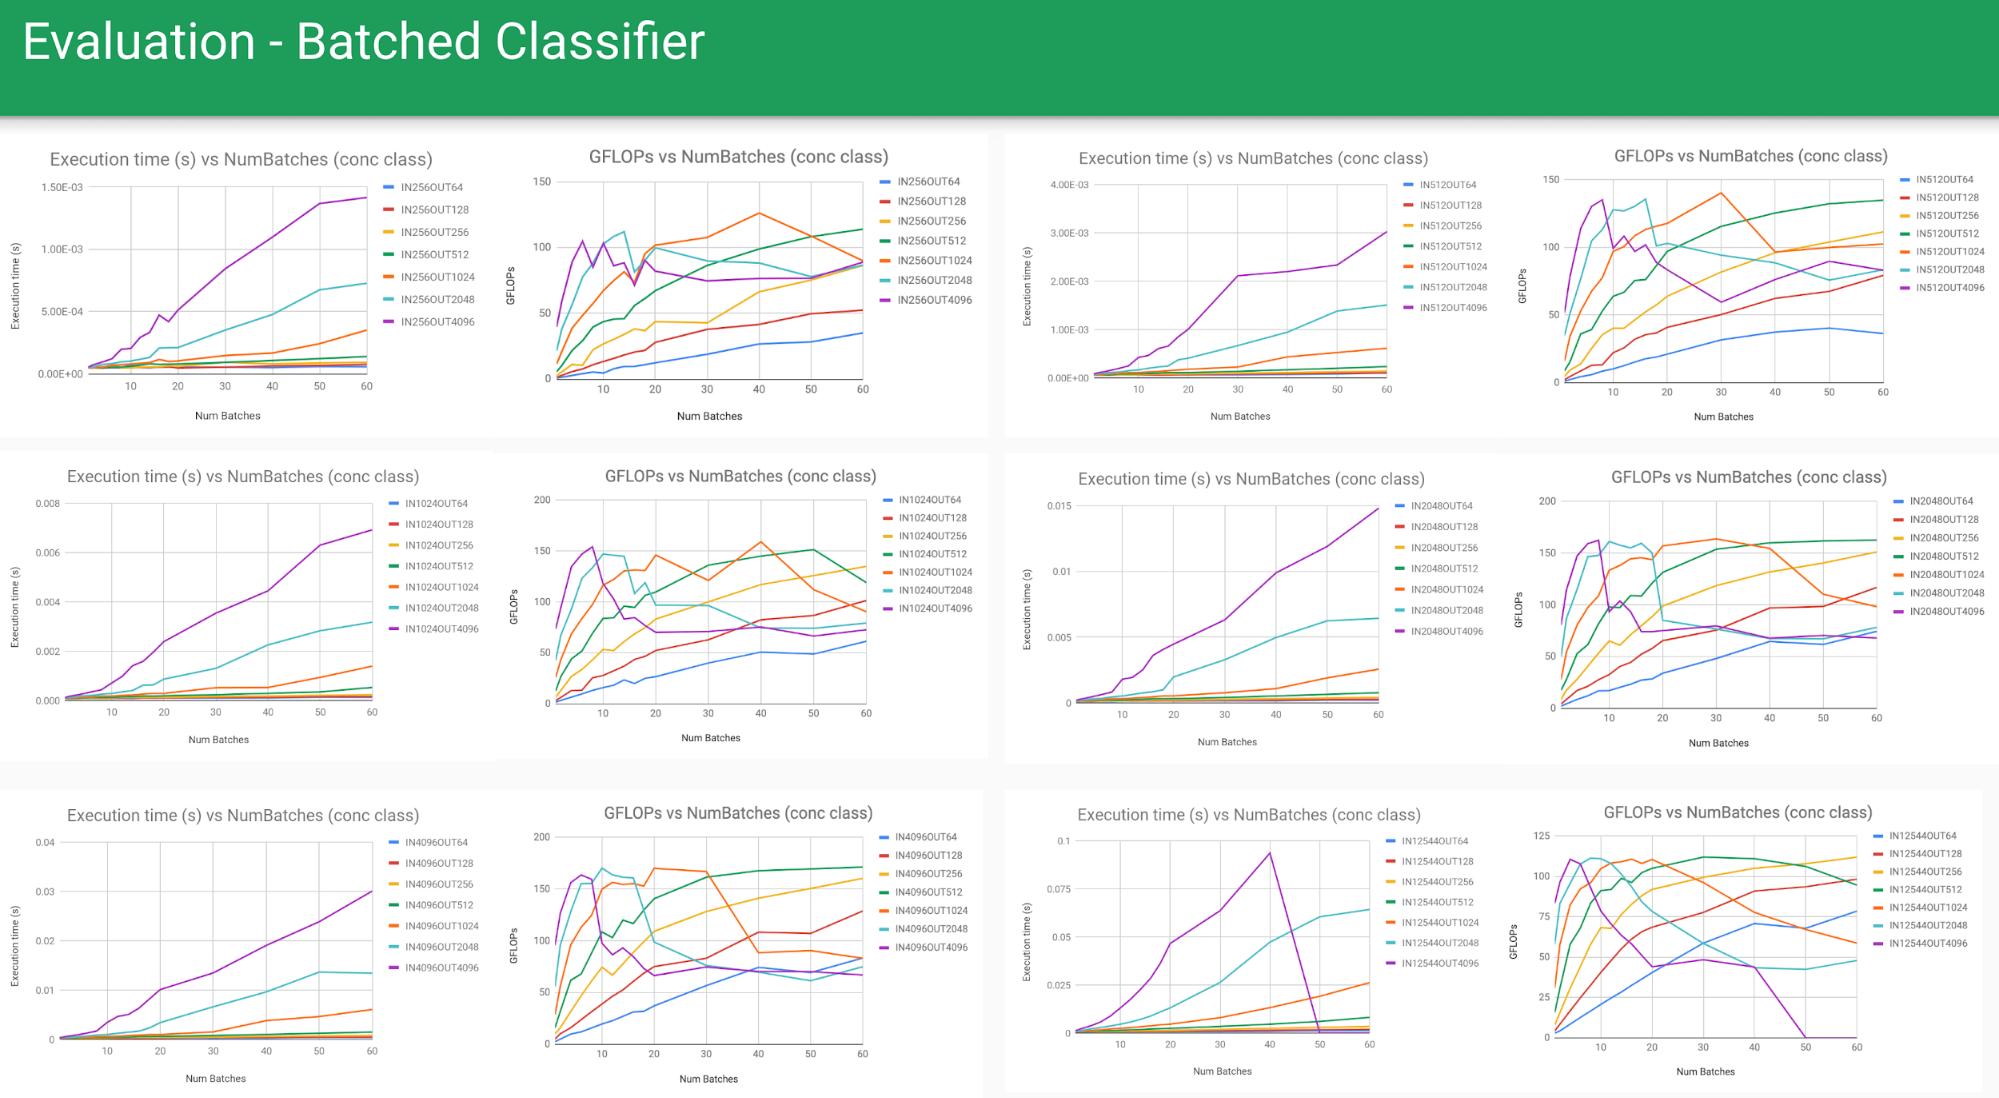
\includegraphics[width=\textwidth]{img/batch-class}
  \caption{Batched classifier performance.}
\end{figure}

\newpage~\newpage
\subsection{AWS M60 GPU Graphs}
\begin{figure}[htb]
  \centering
  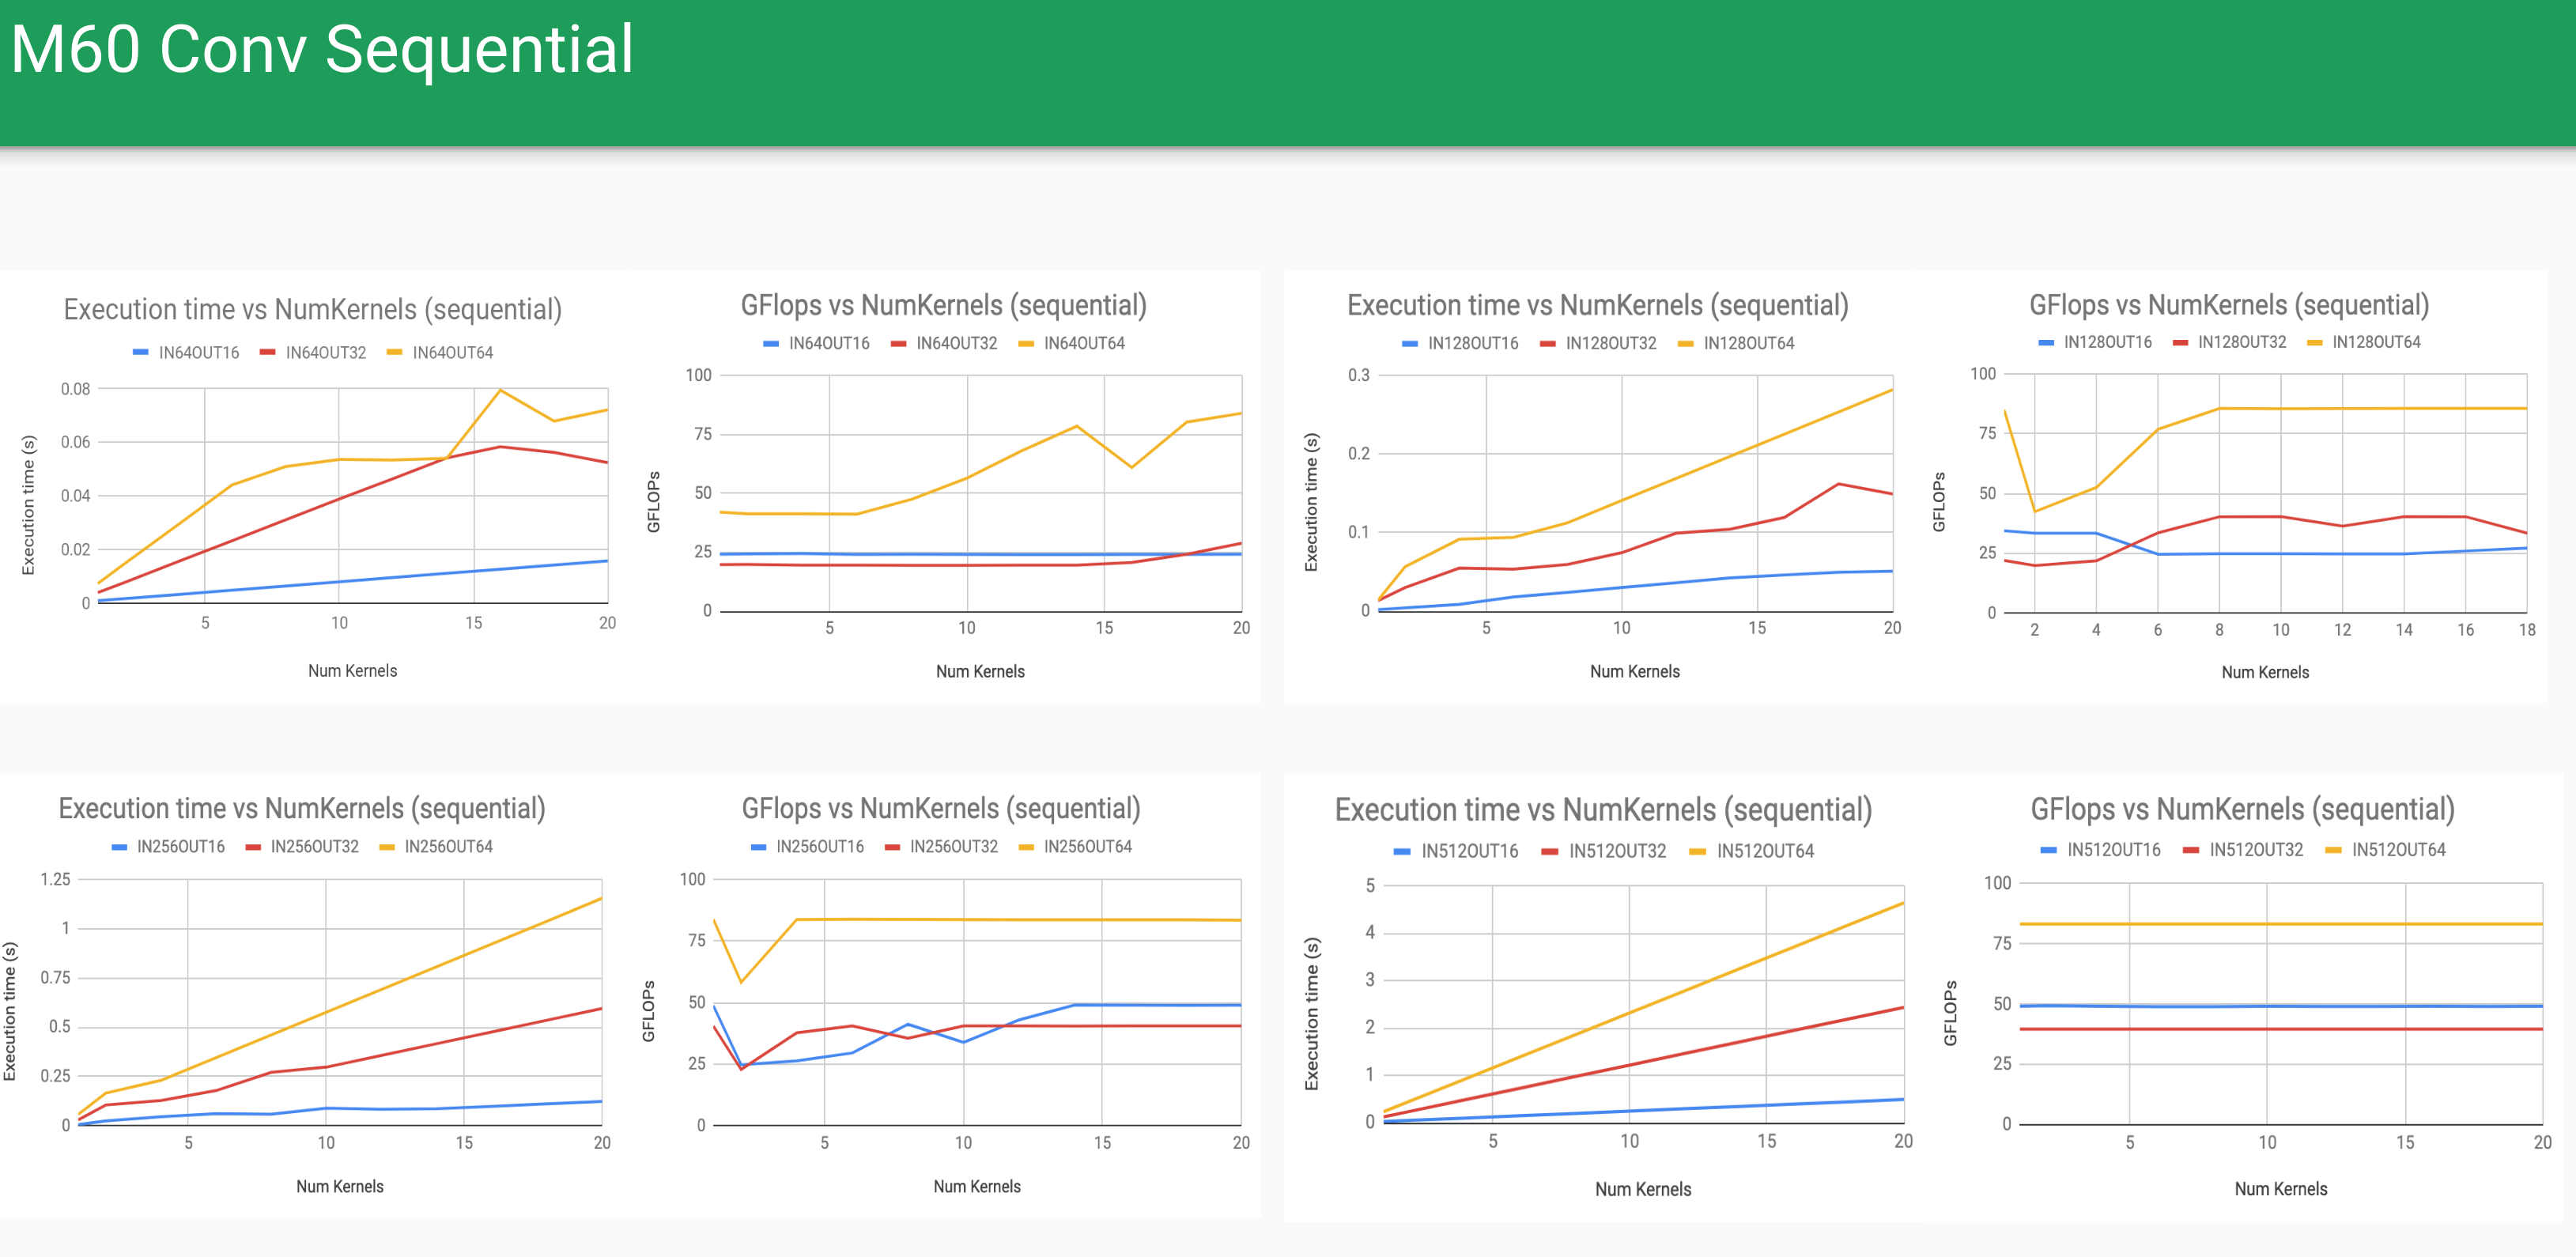
\includegraphics[width=\textwidth]{img/m60-seq-conv}
  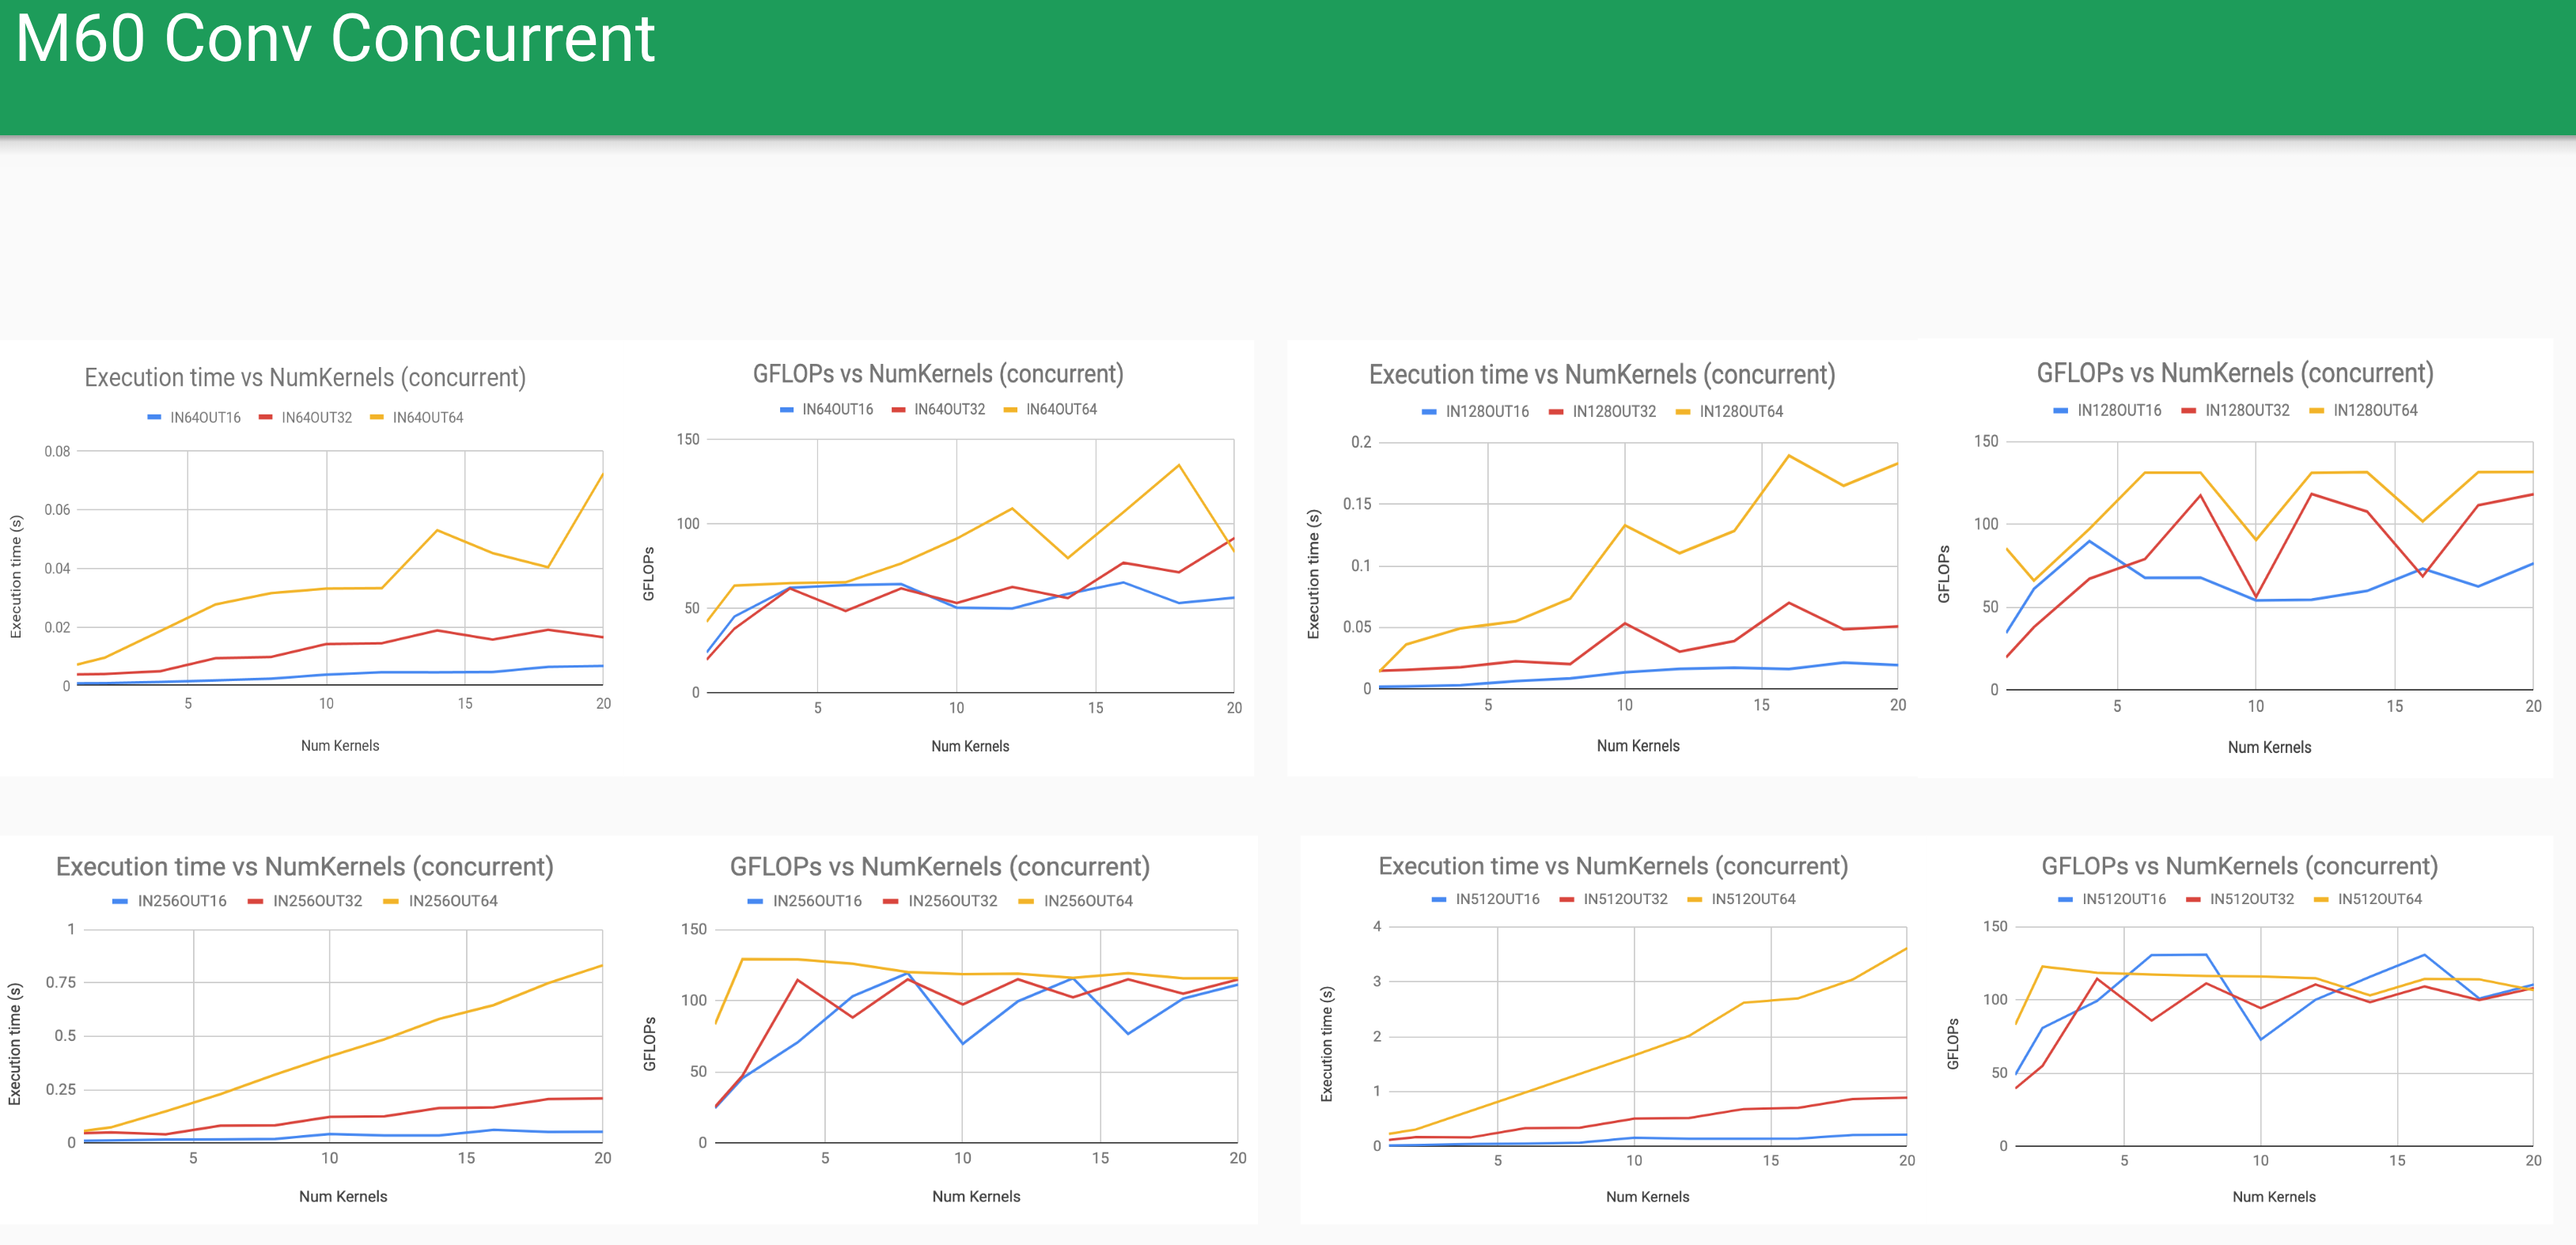
\includegraphics[width=\textwidth]{img/m60-conc-conv}
  \caption{Sequential and concurrent convolution performance.}
\end{figure}

\newpage~\newpage
\begin{figure}[htb]
  \centering
  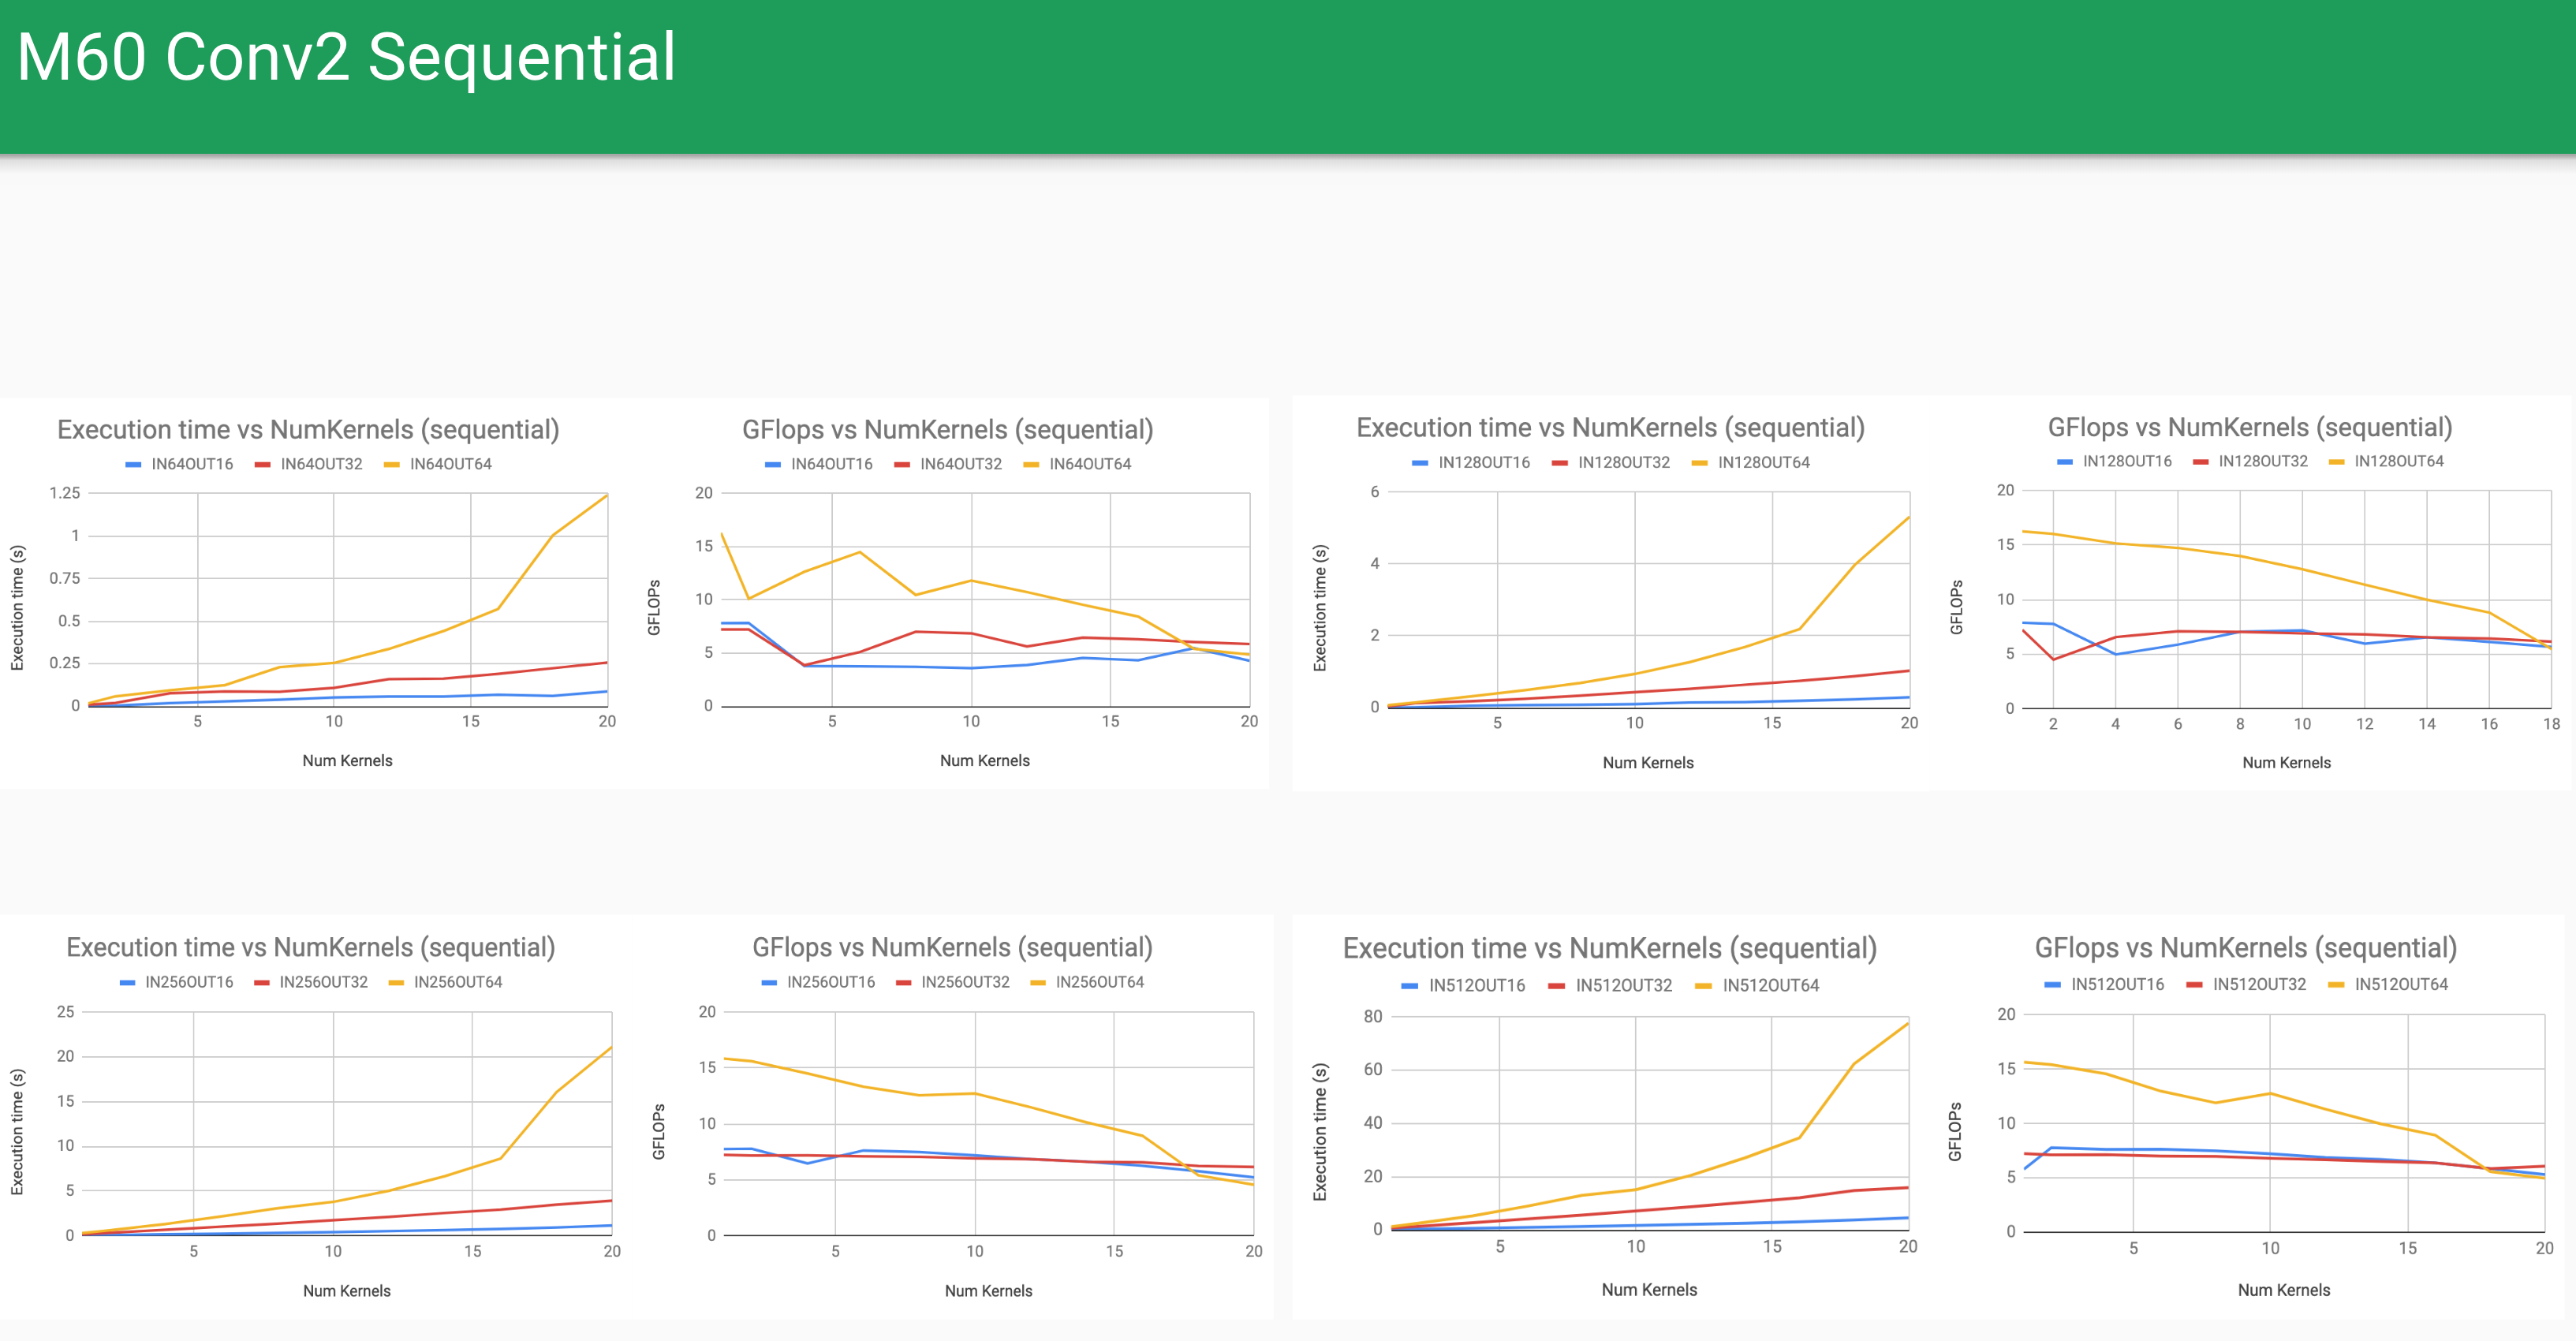
\includegraphics[width=\textwidth]{img/m60-seq-conv2}
  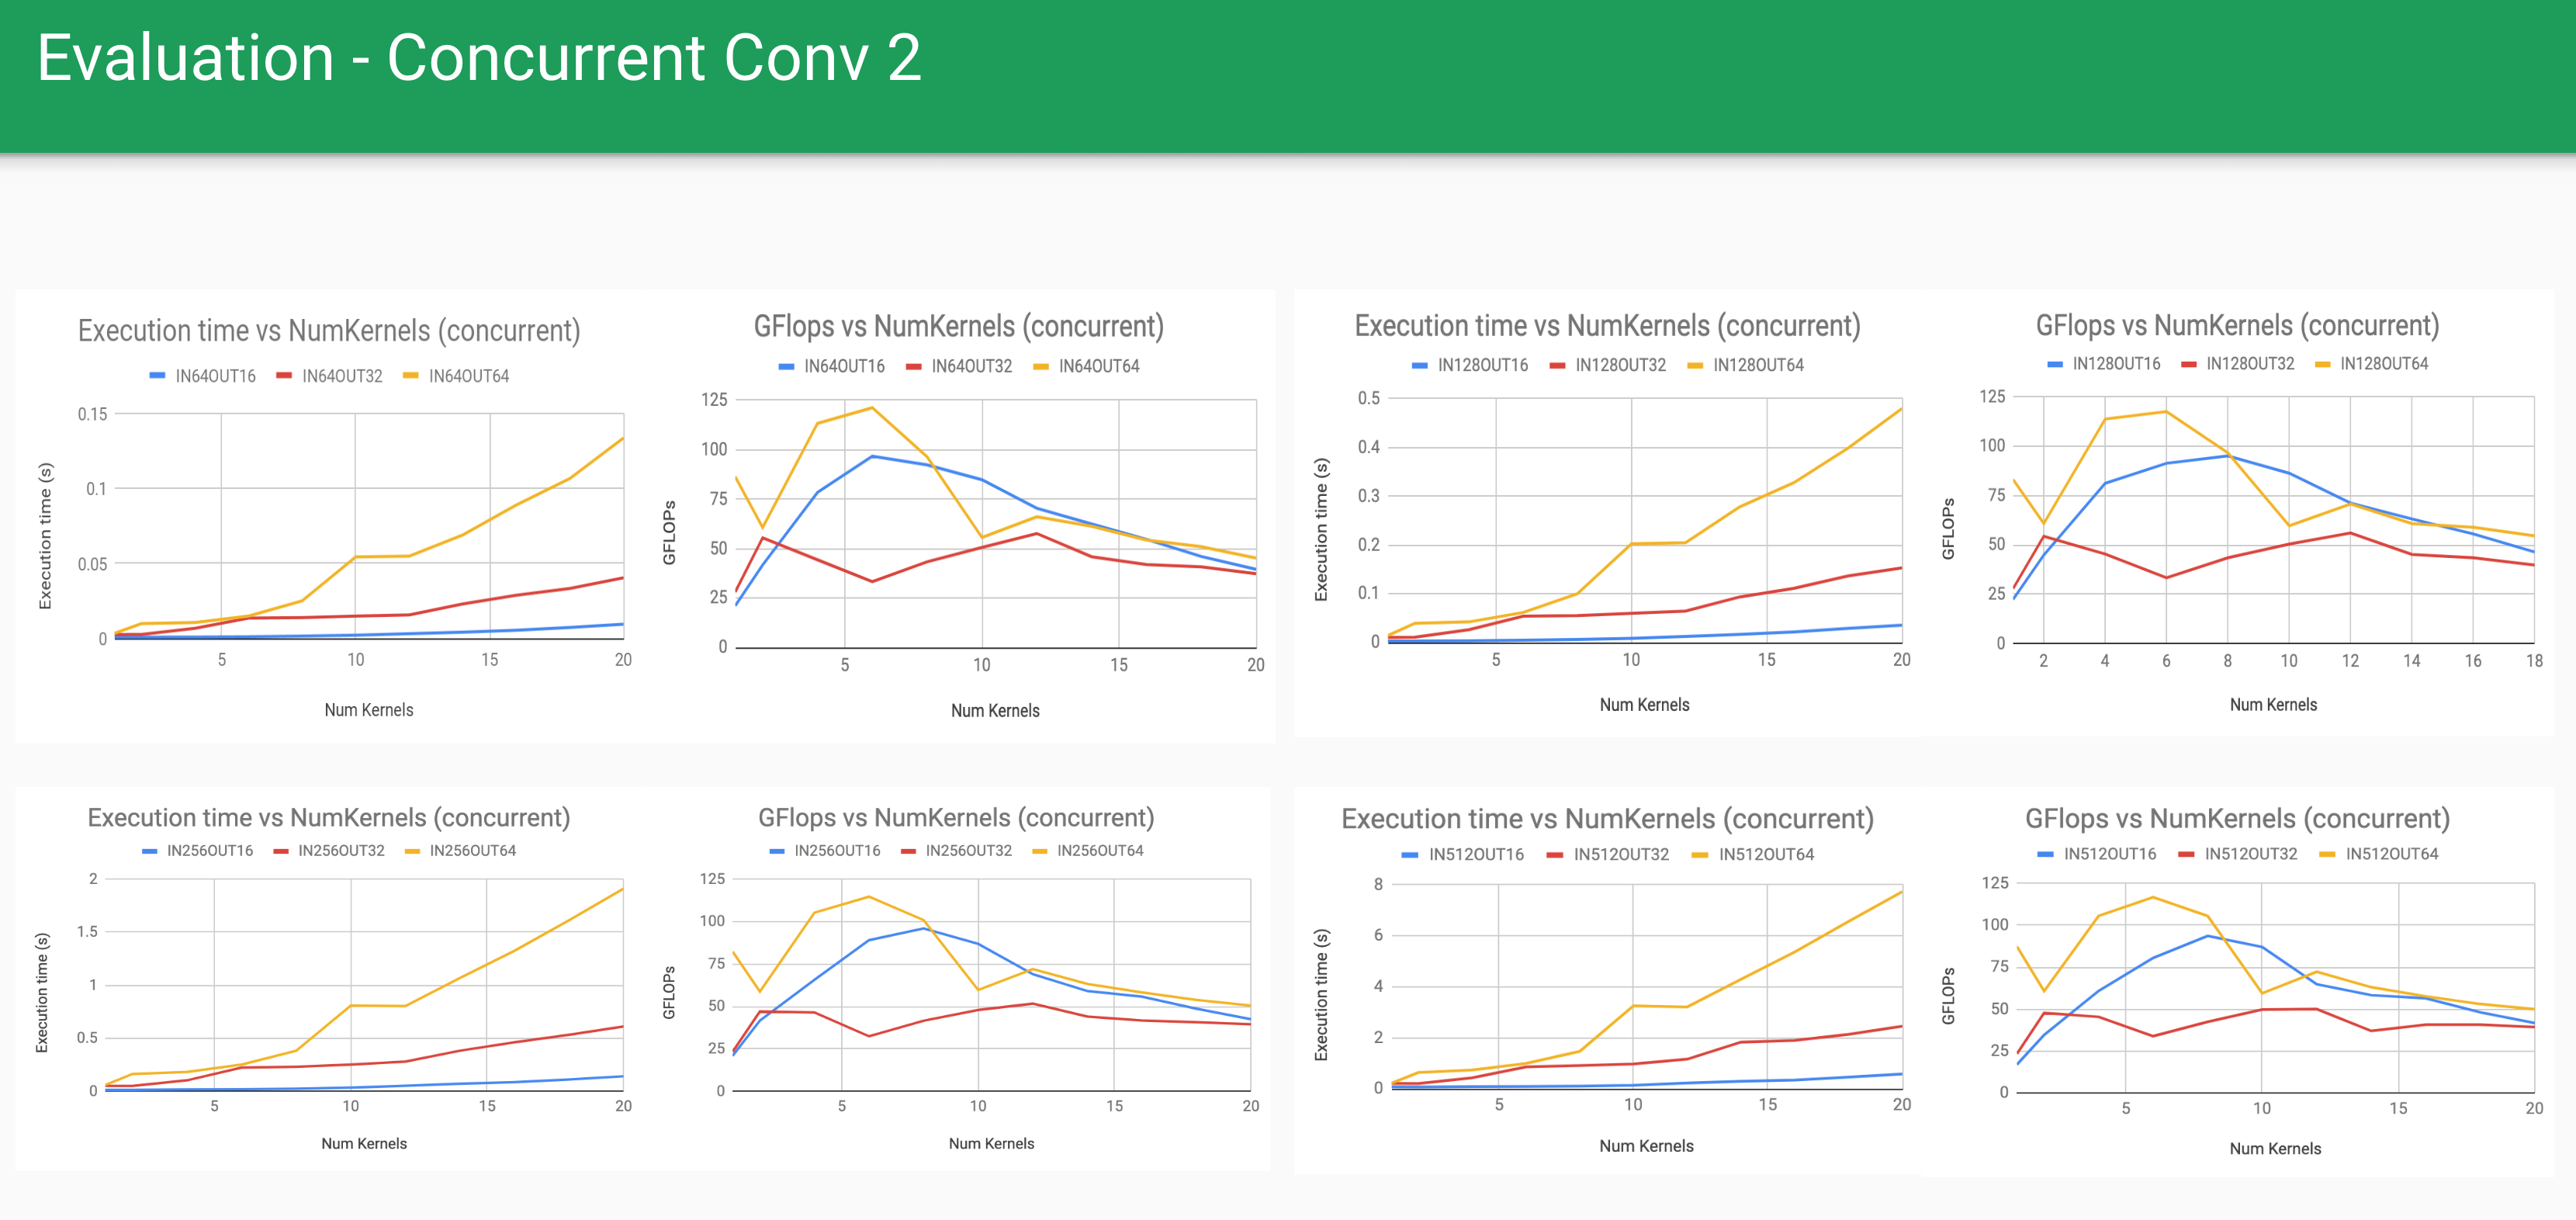
\includegraphics[width=\textwidth]{img/m60-conc-conv2}
  \caption{Sequential and concurrent convolution 2 performance.}
\end{figure}

\newpage~\newpage
\begin{figure}[htb]
  \centering
  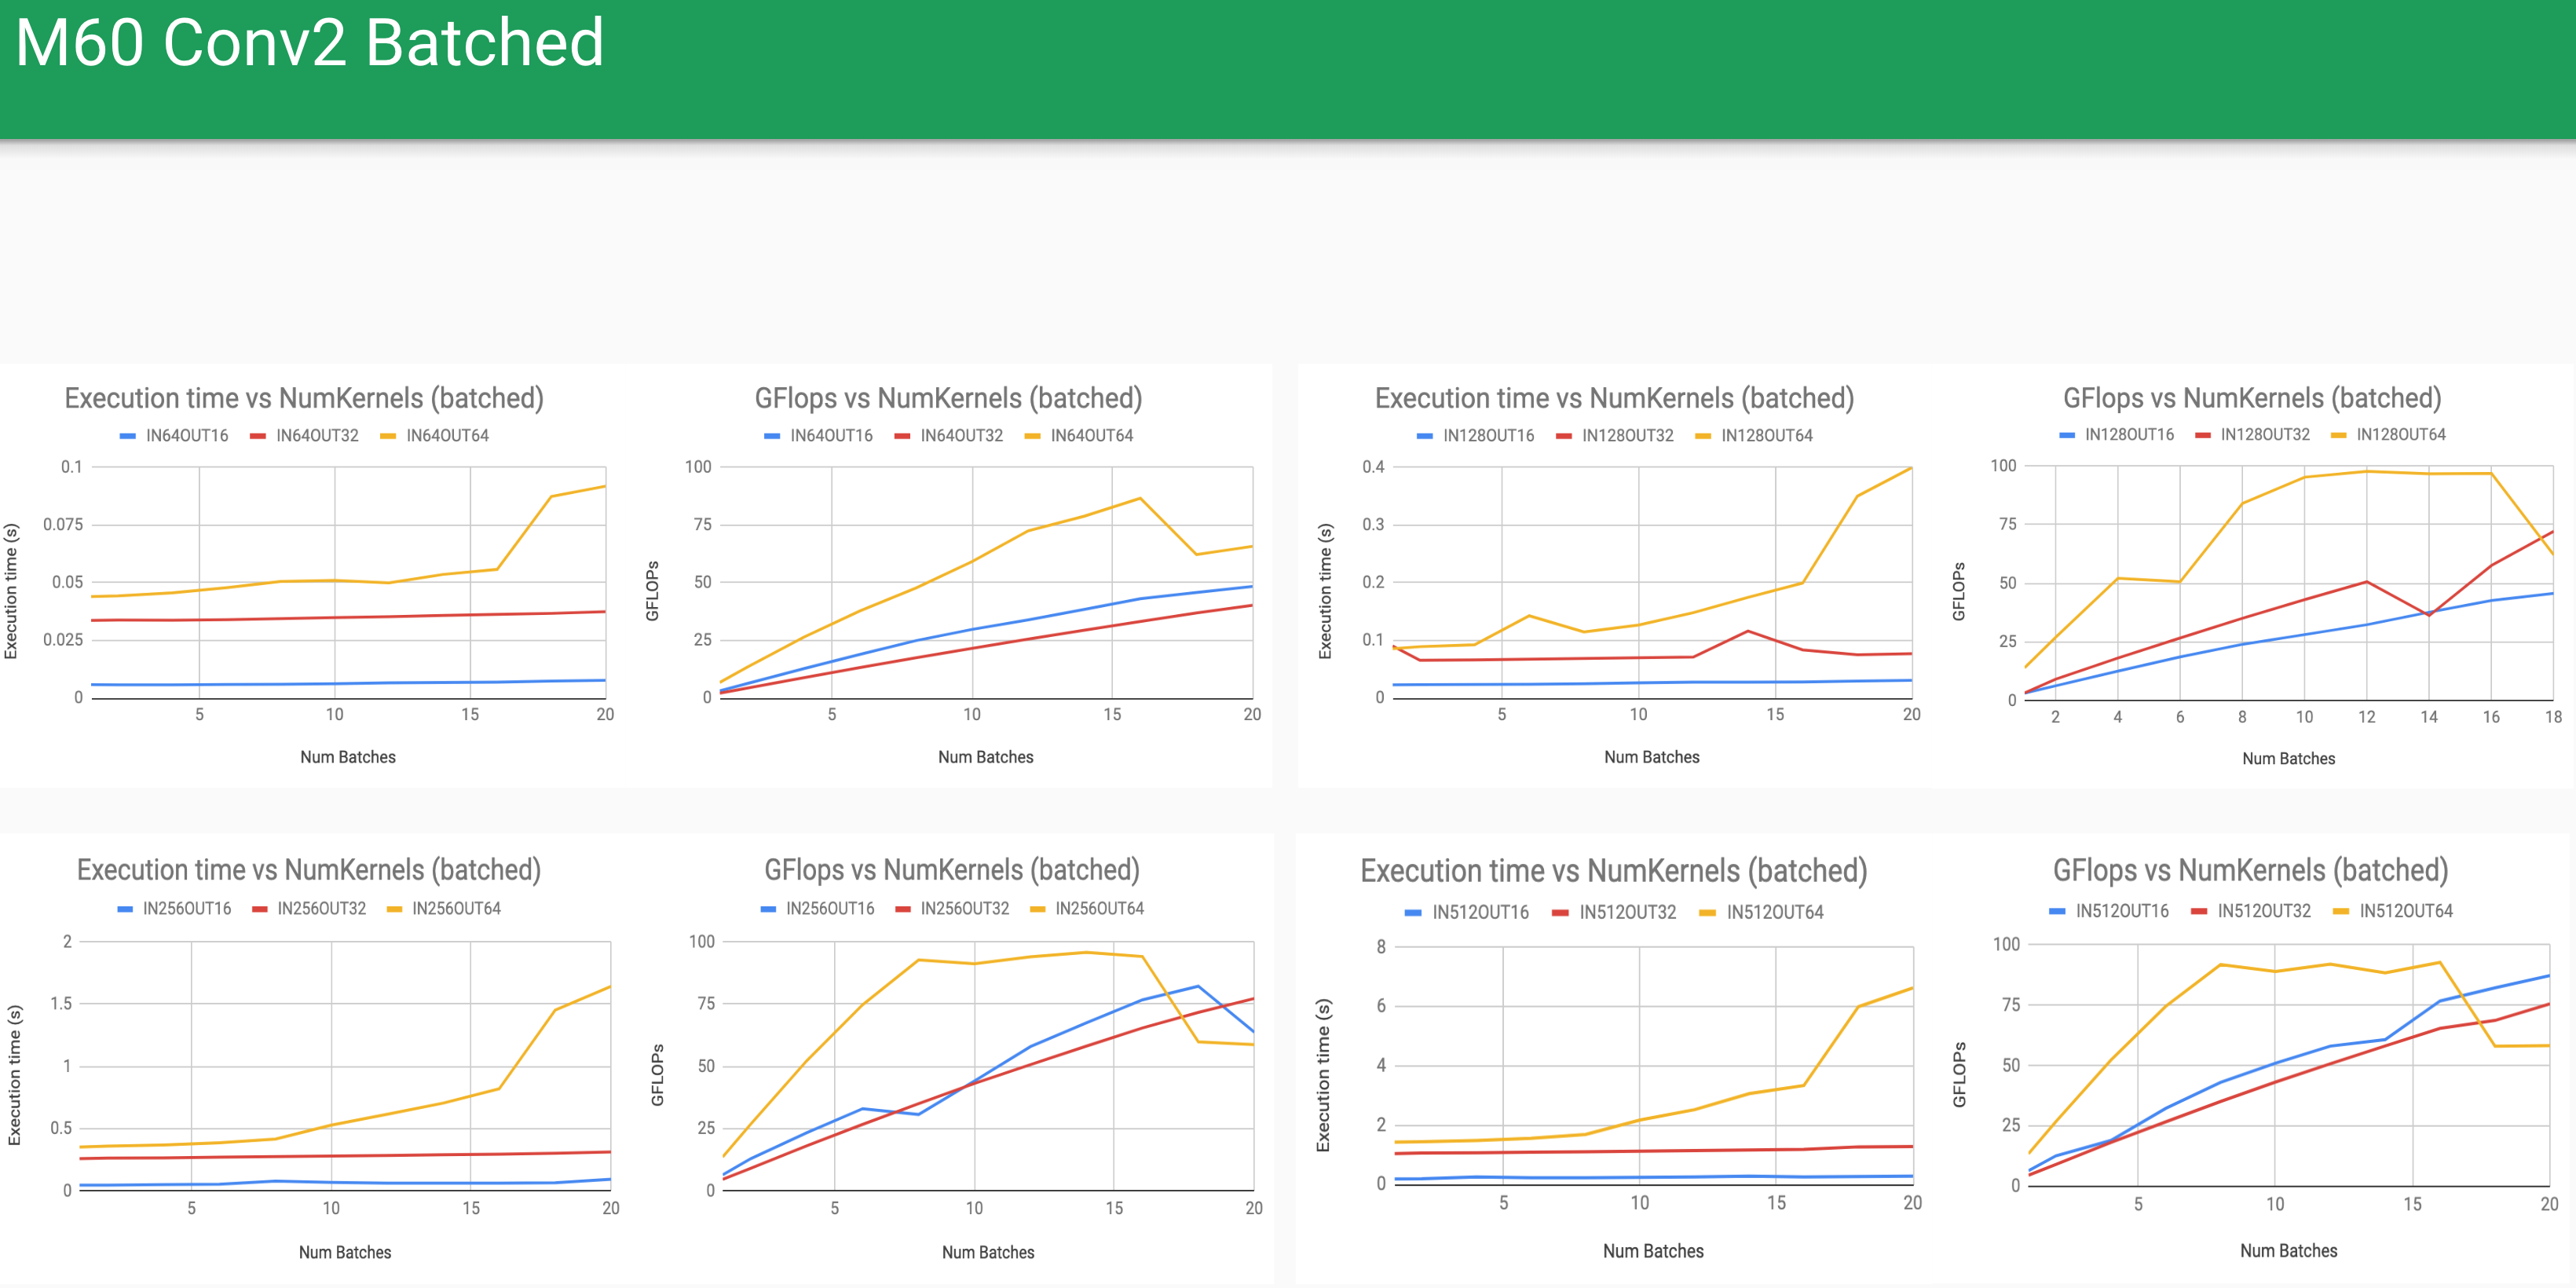
\includegraphics[width=\textwidth]{img/m60-batch-conv2}
  \caption{Batched convolution 2 performance.}
\end{figure}

\newpage~\newpage
\begin{figure}[htb]
  \centering
  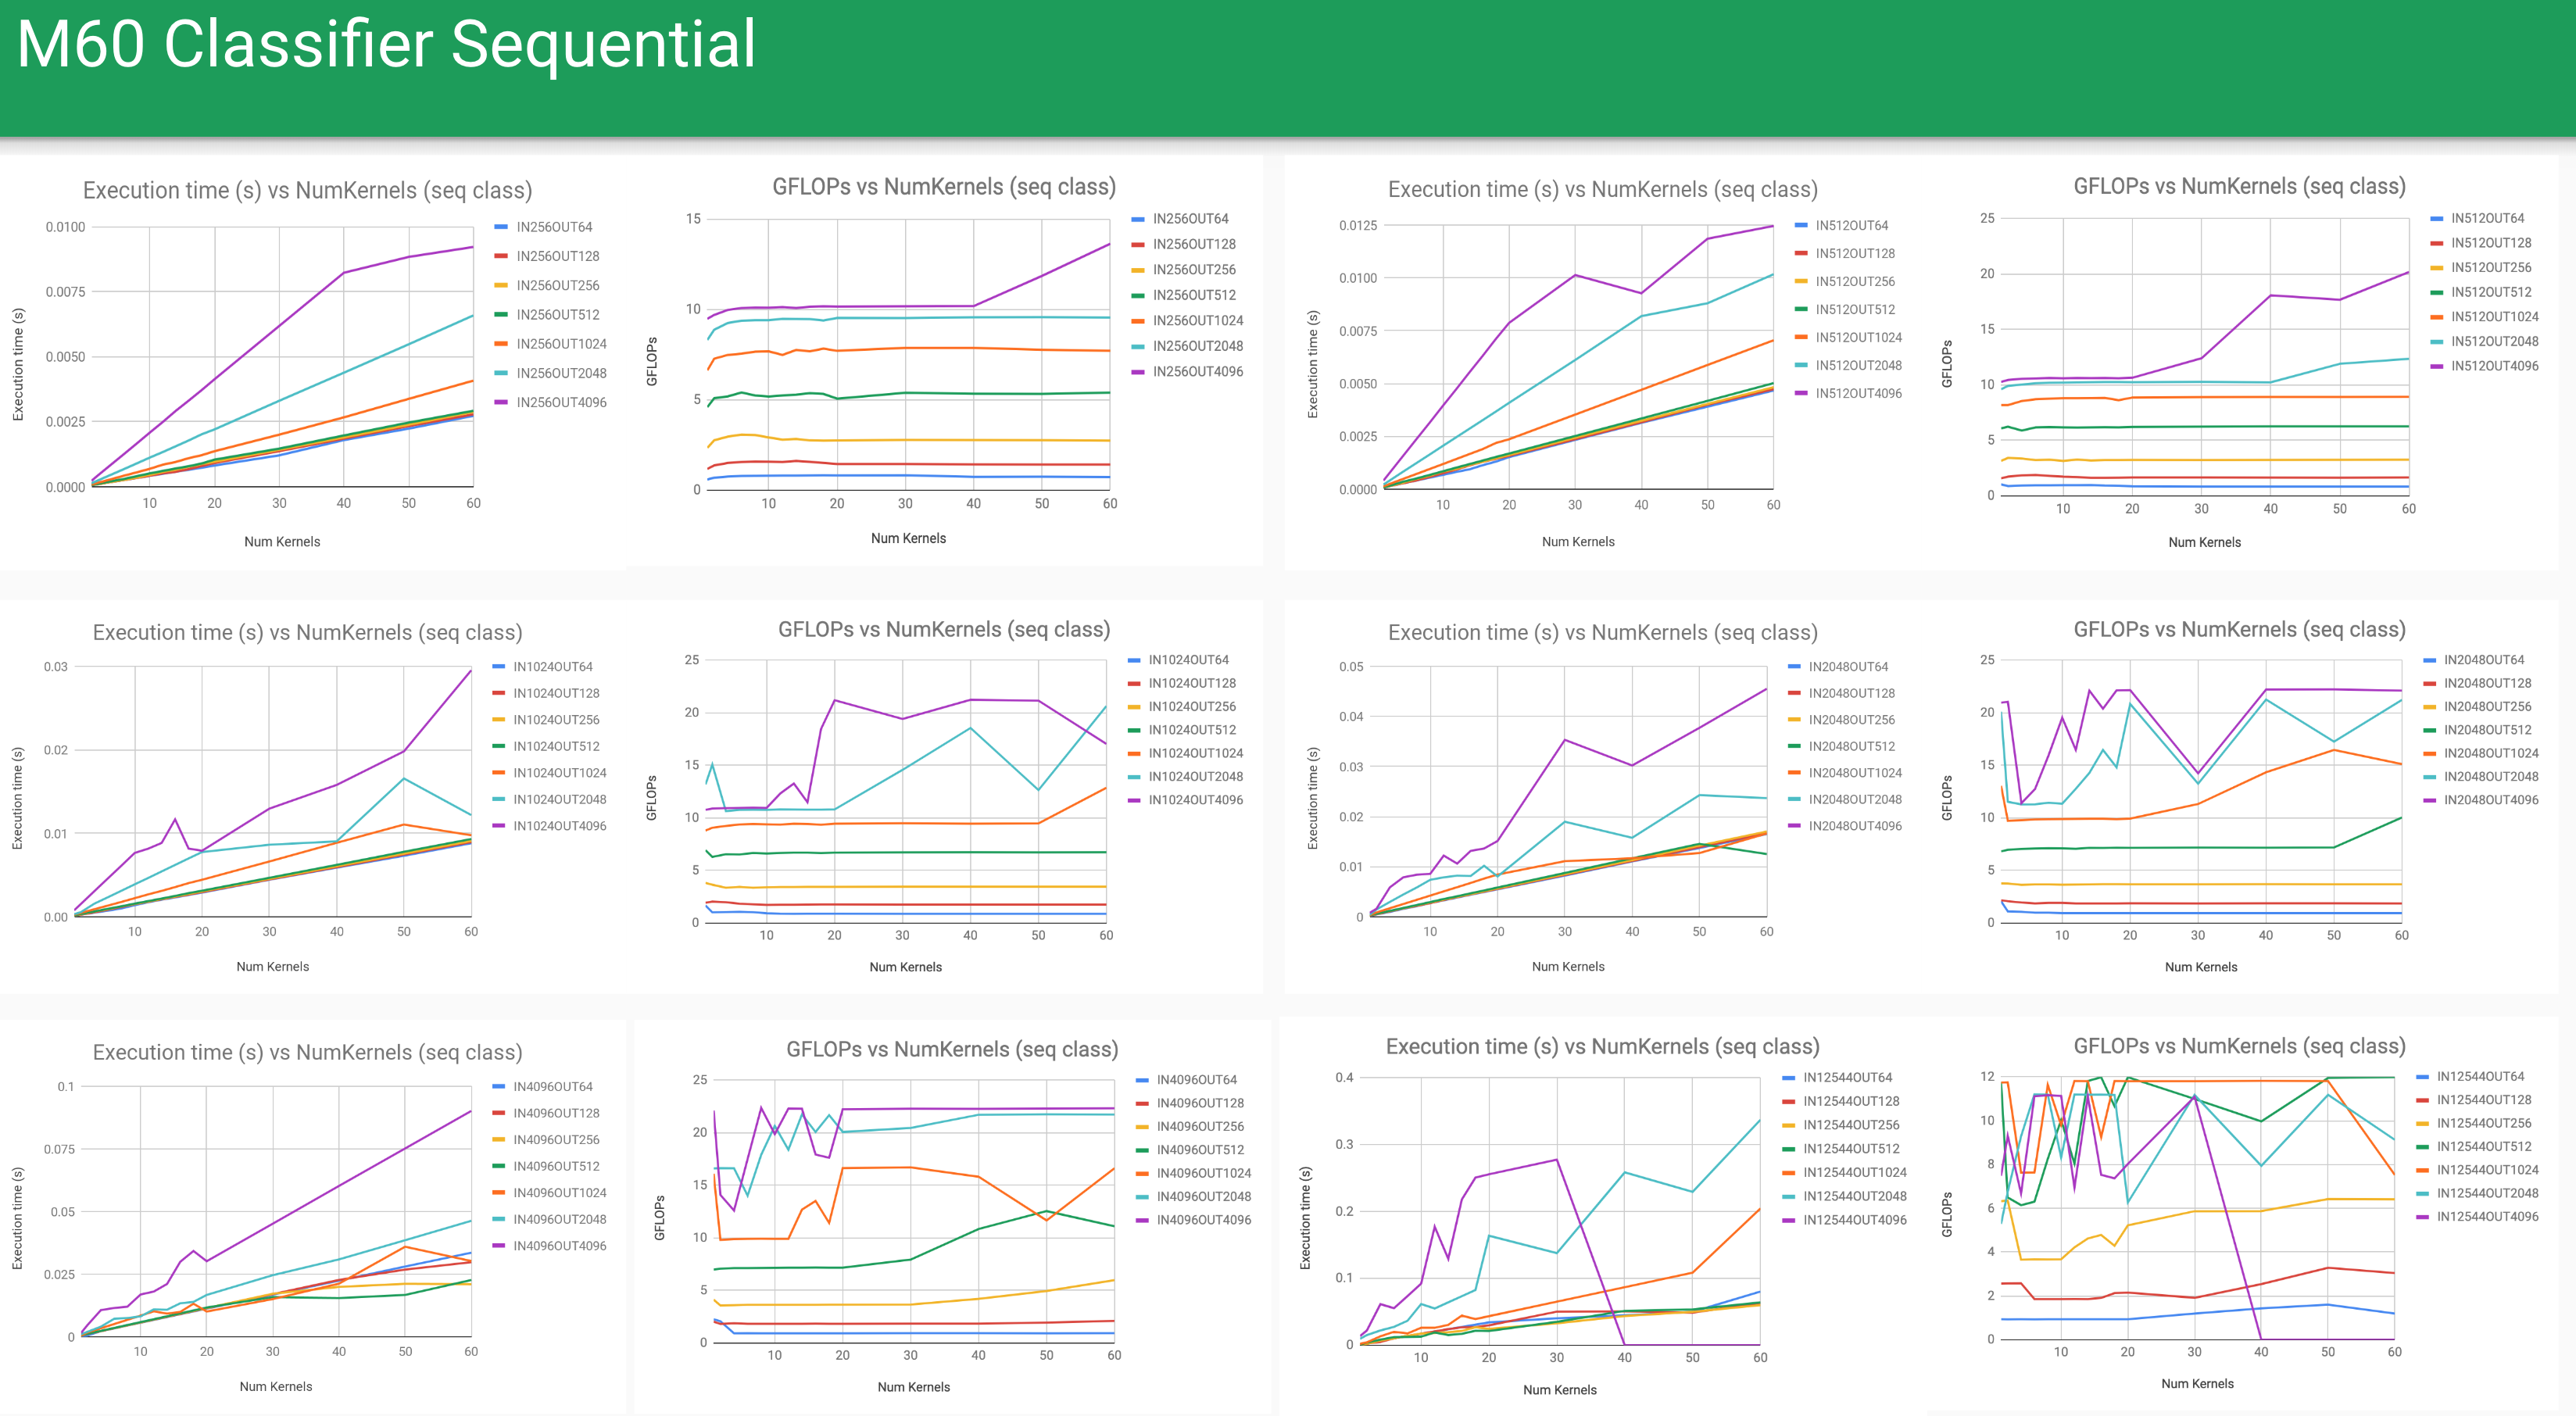
\includegraphics[width=\textwidth]{img/m60-seq-class}
  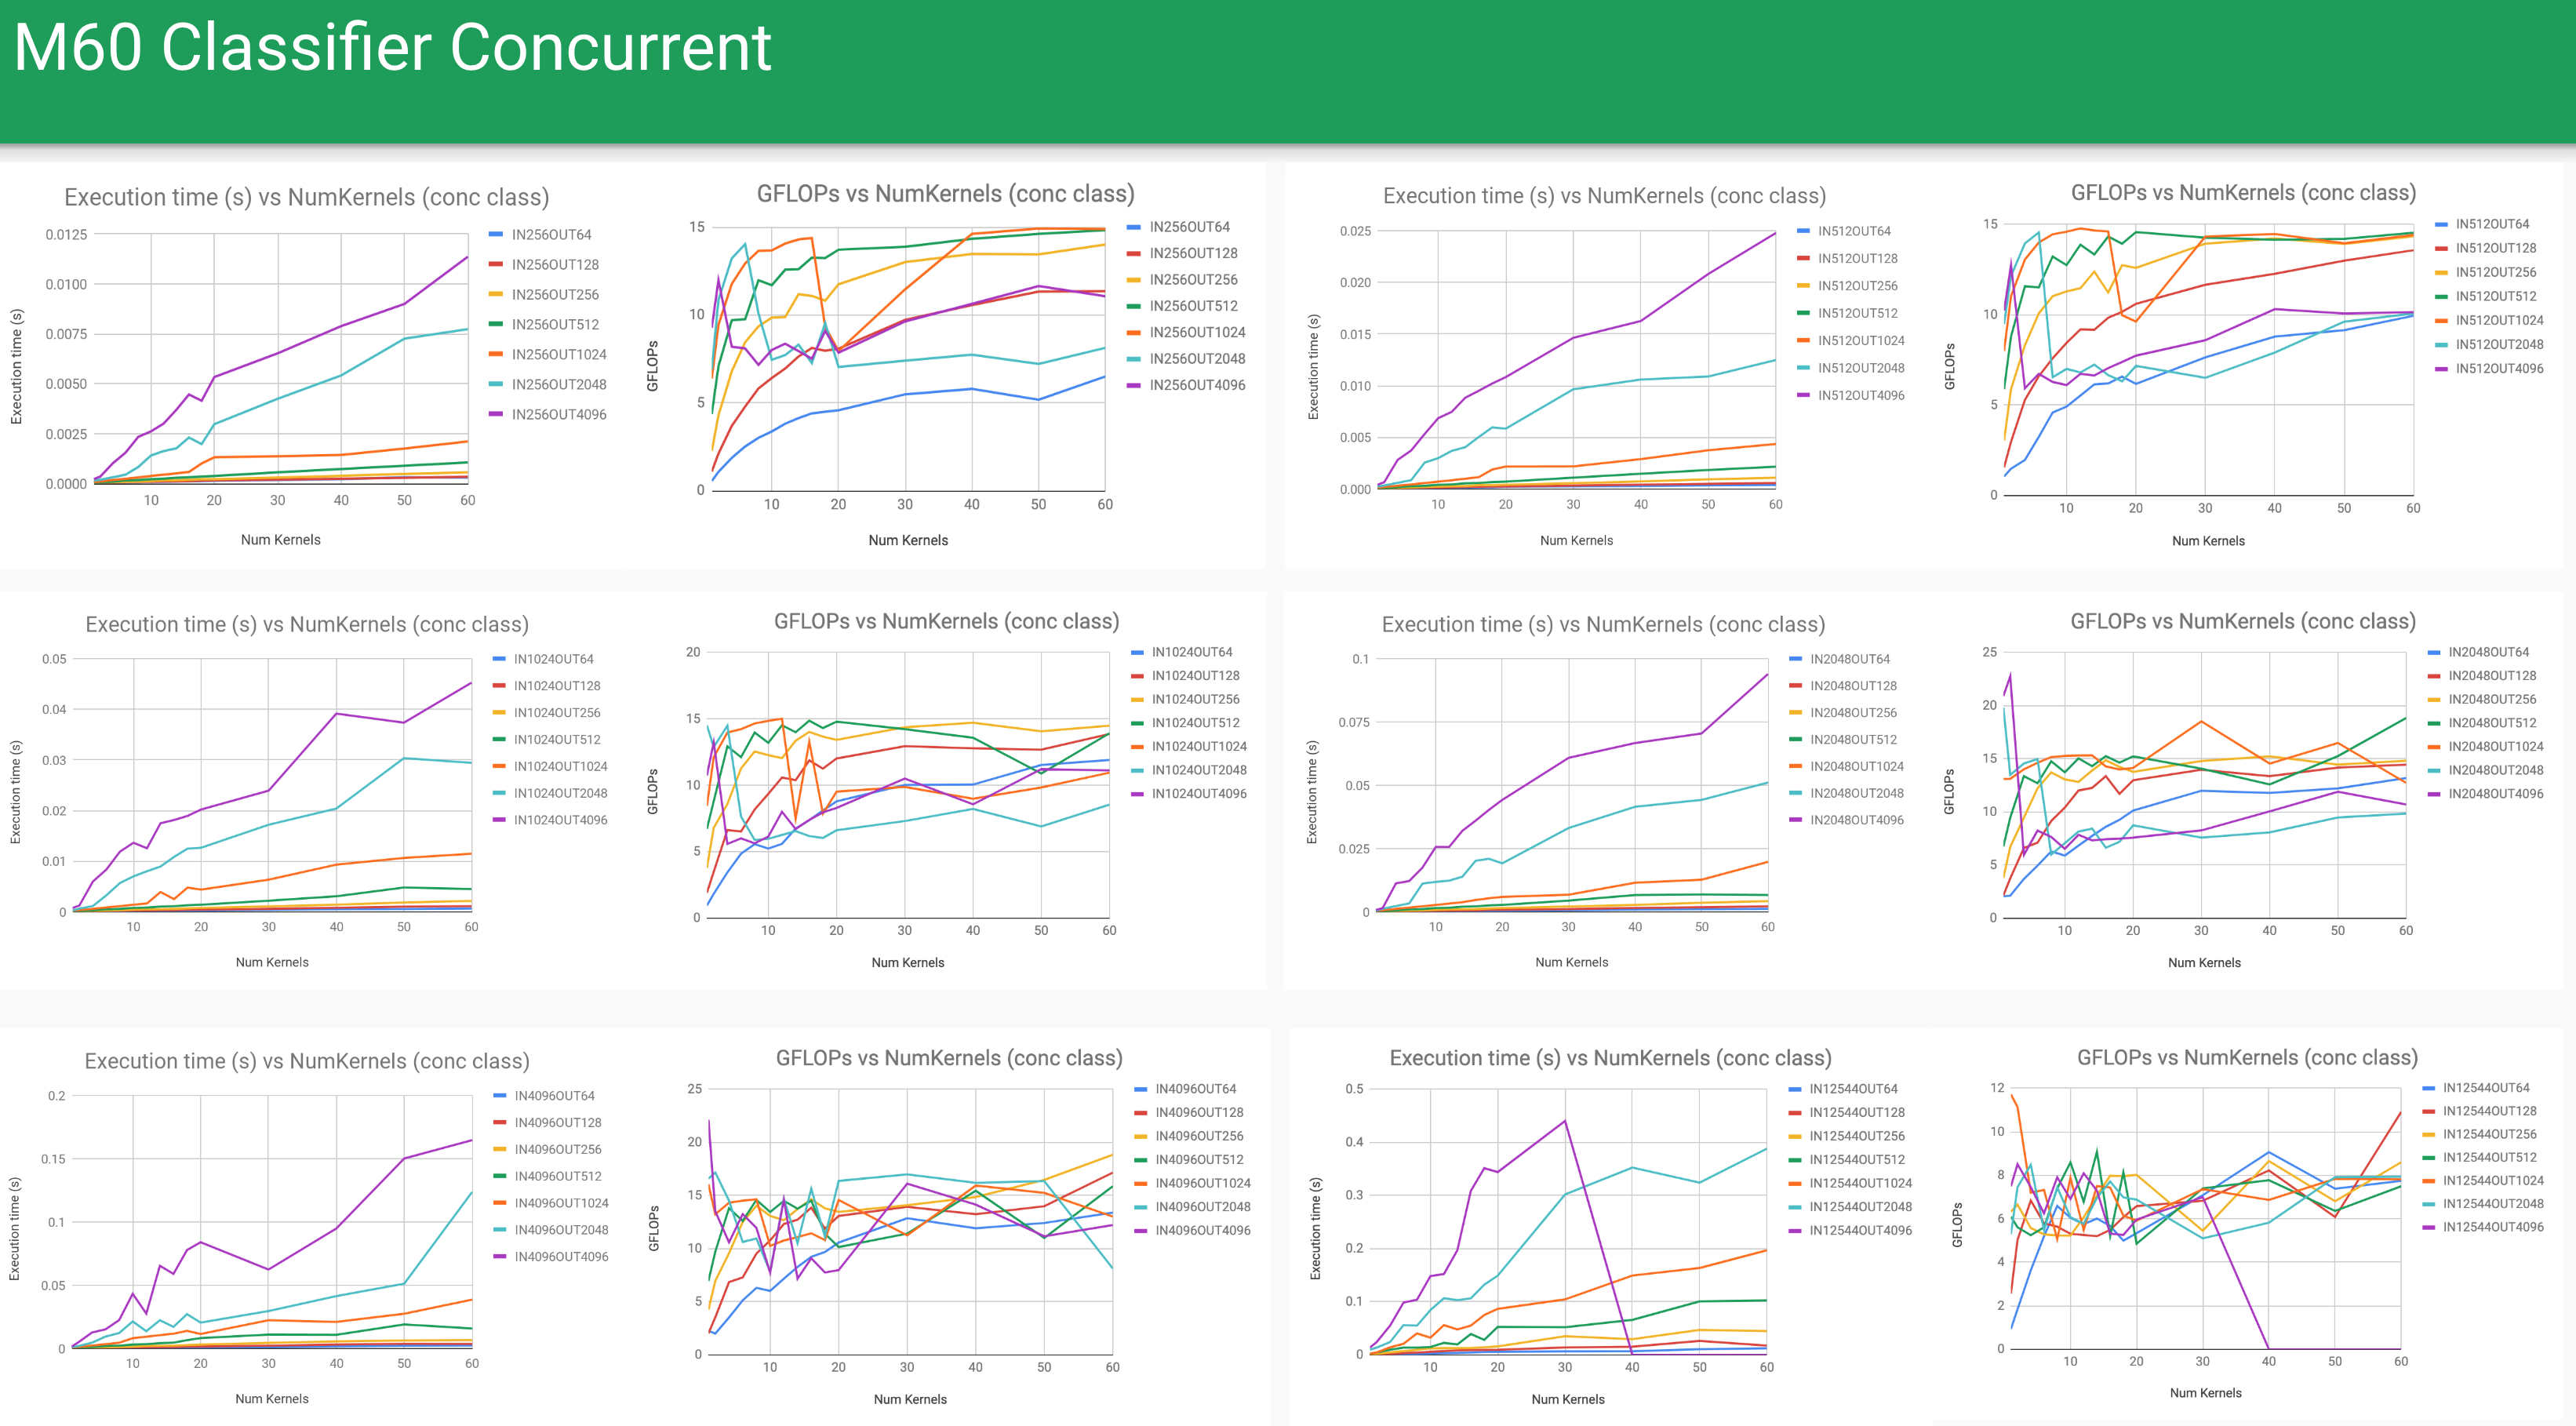
\includegraphics[width=\textwidth]{img/m60-conc-class}
  \caption{Sequential and concurrent classifier performance.}
\end{figure}

\newpage~\newpage
\begin{figure}[htb]
  \centering
  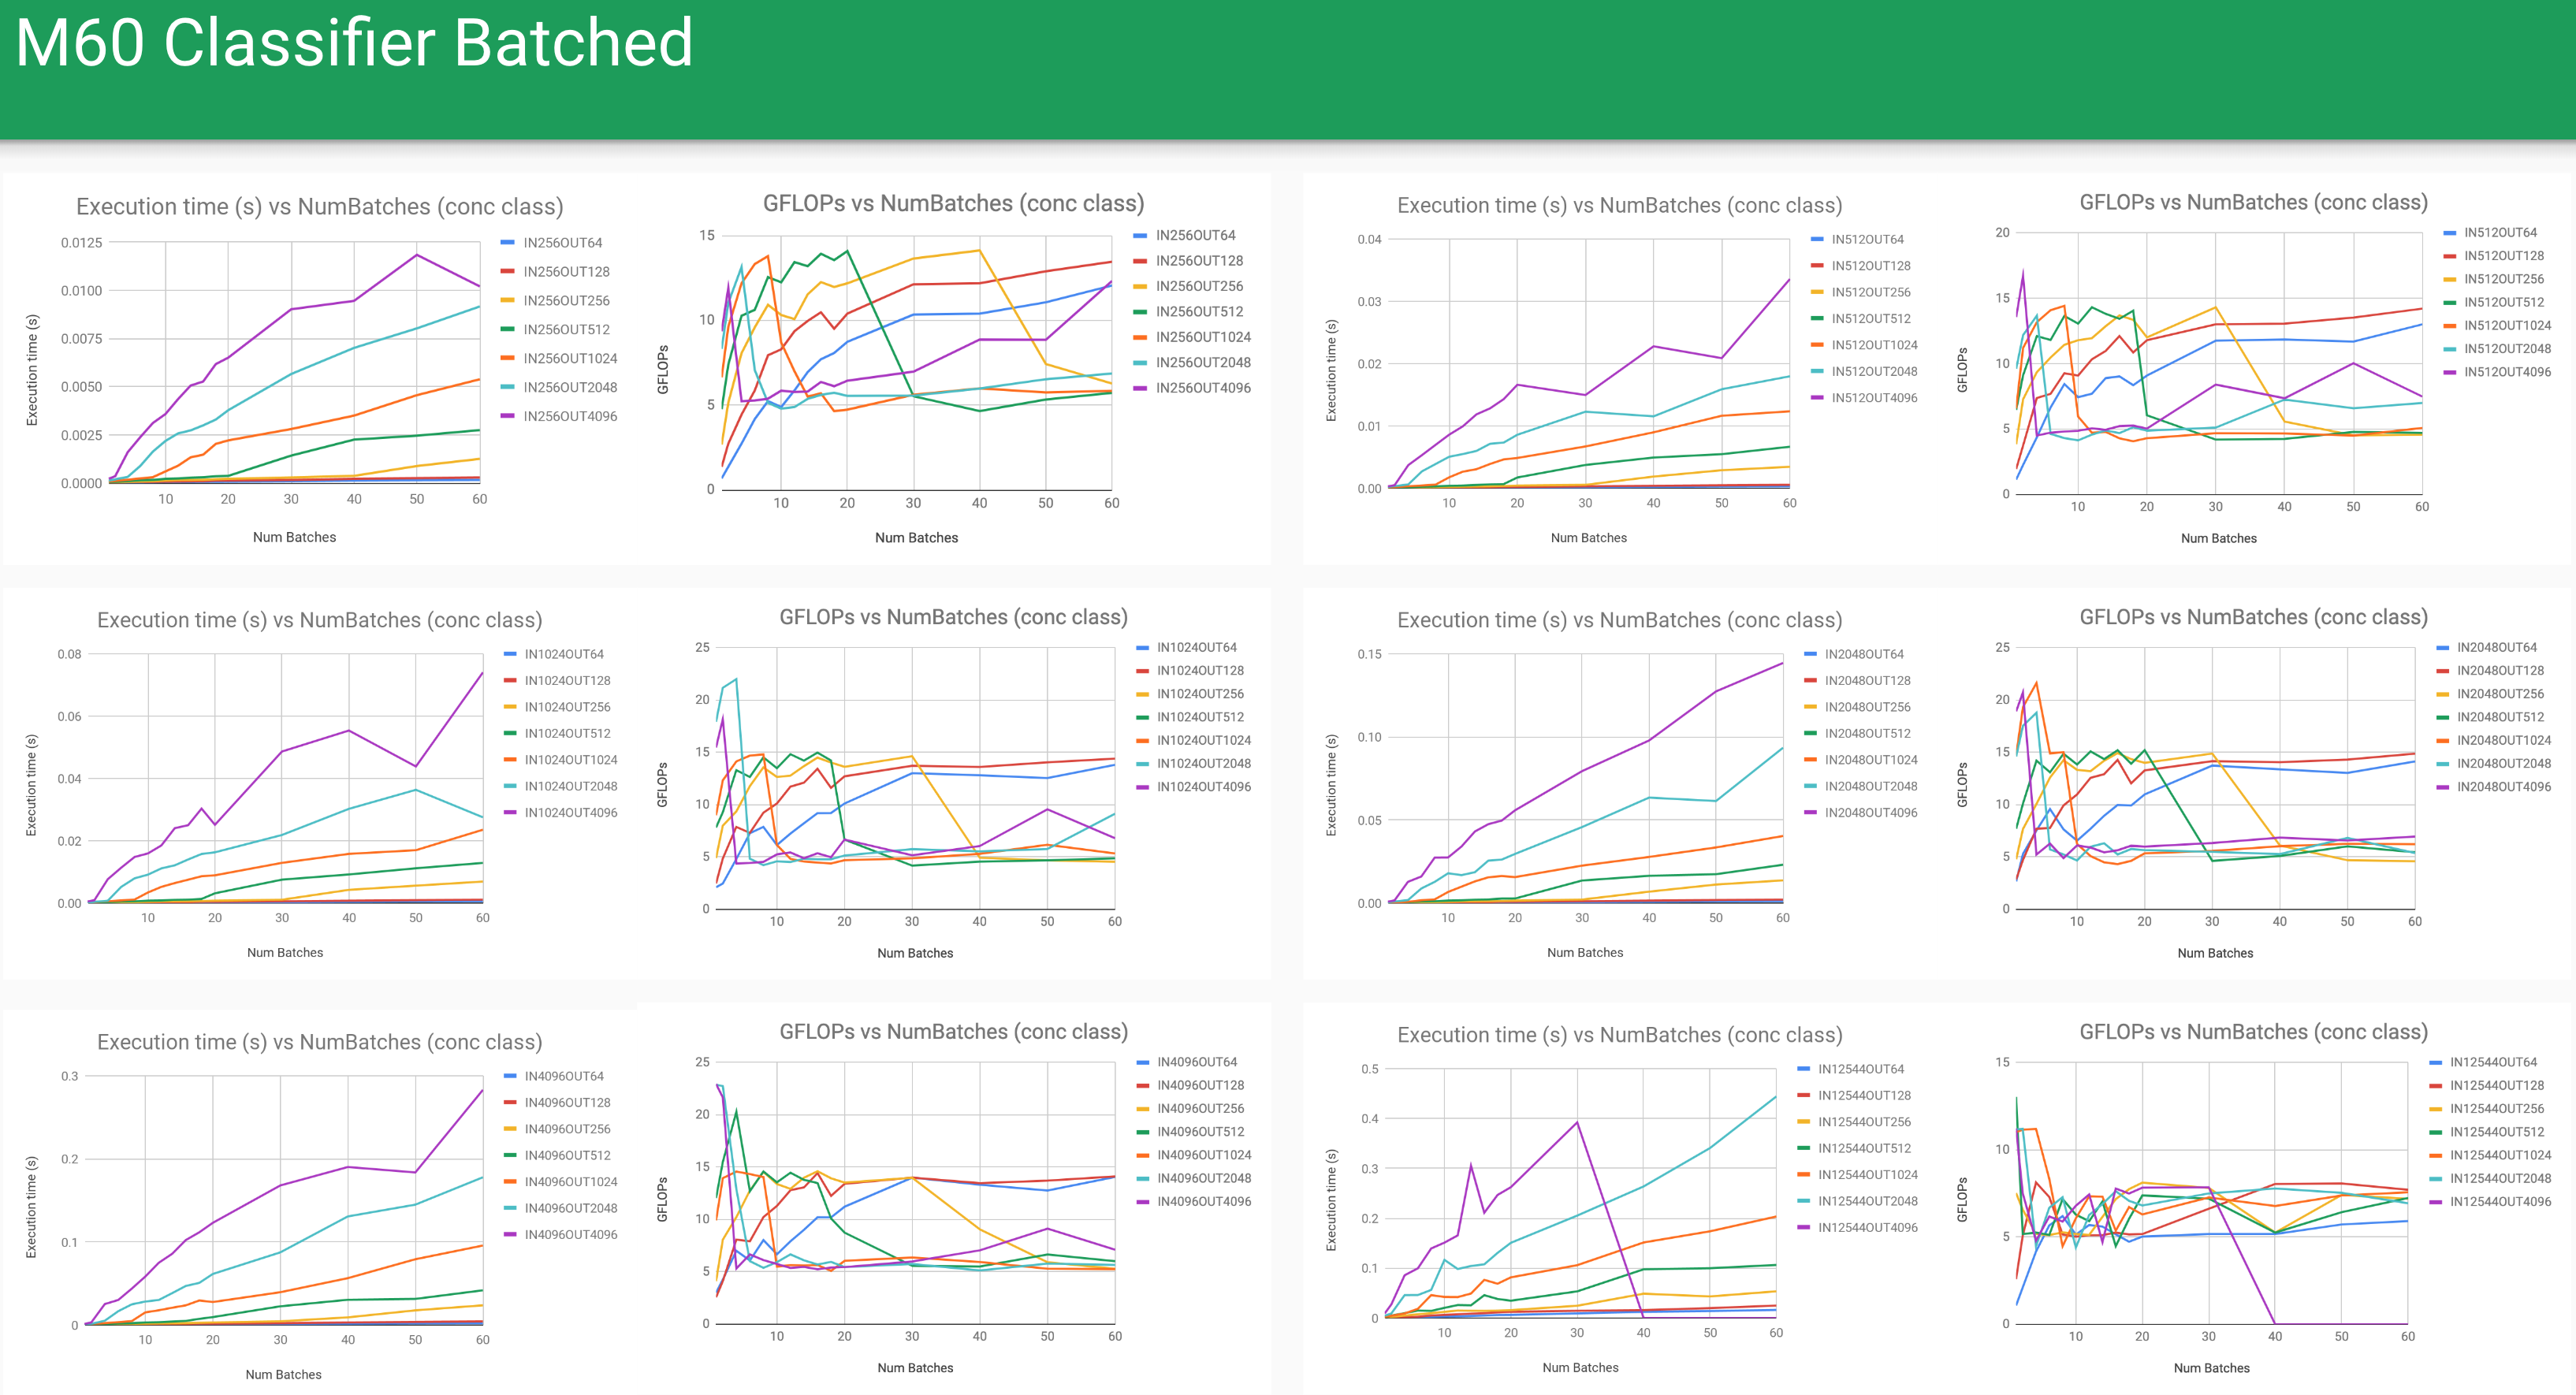
\includegraphics[width=\textwidth]{img/m60-batch-class}
  \caption{Batched classifier performance.}
\end{figure}

\end{document}
\endinput
%%
%% End of file `sample-sigconf.tex'.
